\documentclass[12pt]{report}

\usepackage[utf8]{inputenc}
\usepackage[T1]{fontenc}
\usepackage{lmodern}
\usepackage[catalan]{babel}
\usepackage{geometry}
\usepackage{hyperref}
\usepackage{xcolor}
\usepackage{booktabs}
\usepackage{multirow}
\usepackage[catalan]{todonotes}
\usepackage[bf,sf,small, pagestyles]{titlesec} % Format dels títols de secció
\usepackage[font={footnotesize, sf}, labelfont=bf]{caption} % Format dels peus de figura
\usepackage{graphicx}
\usepackage{amsmath, amssymb, xfrac}
\usepackage{siunitx}
\usepackage[siunitx]{circuitikz}
\usepackage[catalan, sort]{cleveref}

% Marges, etc
\geometry{
	a4paper,
	right = 2.5cm,
	left = 2.5cm,
	bottom = 3cm,
	top = 3cm,
	columnsep = 1cm,
	twoside
}
\setlength{\parskip}{0pt}

% Referències
\hypersetup{
	colorlinks,
	linkcolor = {red!50!blue},
	linktoc = page
}
\crefname{figure}{figura}{figures}

% Figures
\graphicspath{{./informe-2/figs/} {./informe-3/figs/} {./informe-4/figs/} {./informe-5/figs/} {./informe-7/figs/} {./annexos/figs/}}

% Peus de pàgina
\newpagestyle{pagina}{
	\headrule
	\sethead*{}{}{\sffamily {\slshape Informe \thechapter: }\chaptertitle}
	\footrule
	\setfoot*{}{}{\sffamily \thepage}
}
\renewpagestyle{plain}{
	\footrule
	\setfoot*{}{}{\sffamily \thepage}
}
\pagestyle{pagina}

% Format del títol
\titleformat{\chapter}[display]{\centering \bfseries \sffamily \LARGE}{\large \sf Informe \thechapter}{4pt}{}{\thispagestyle{pagina}}
\titlespacing{\chapter}{0pt}{*2}{*4}

% Unitats
\sisetup{
	inter-unit-product = \ensuremath{ \, },
	allow-number-unit-breaks = true,
	detect-family = true,
	list-final-separator = { i },
	list-units = single,
	separate-uncertainty = true
}
% Valor amb incertesa
\newcommand{\data}[3]{\SI{#1 \pm #2}{#3}}
\renewcommand{\vec}[1]{\mathbf{#1}}
\newcommand{\abs}[1]{\left\lvert #1 \right\rvert}
\makeatletter
\newcommand*{\defeq}{\mathrel{\rlap{%
    \raisebox{0.3ex}{$\m@th\cdot$}}%
  \raisebox{-0.3ex}{$\m@th\cdot$}}%
=
}
\makeatother

% Format de l'abstract
\newlength{\currentparindent}
\newenvironment{resum} 
{ \setlength{\currentparindent}{\parindent} \noindent \begin{center} \begin{minipage}{0.8\linewidth} \setlength{\parindent}{\currentparindent} \footnotesize \slshape }
{ \end{minipage} \end{center}	\vspace{0.5cm} }

% Títol
\title{\sffamily \bfseries Laboratori d'Electromagnetisme}
\author{\sffamily Sandro Barissi, Adrià Marín, Arnau Mas, Robert Prat} 
\date{\sffamily 2018}

% Arxius a incloure
\includeonly{./informe-4/informe-4}

\begin{document}
\maketitle

\newpage
{\sffamily \tableofcontents}
\addcontentsline{toc}{part}{Informes}

% Informes
% Informe 1
\chapter{Representació de camps}
\begin{resum}
	L'objectiu principal d'aquesta pràctica consisteix en representar les línies de camp elèctric i línies equipotencials degudes a tres distribucions de càrrega: un condensador de plaques plano-paral·leles, dos fils infinits i paral·lels i una altra distribució lliure, amb la qual vam estudiar l'efecte punxa. A més, vam analitzar la capacitat del condensador trobant la càrrega per unitat de longitud.

	Els resultats han estat acurats als dos primer casos, trobant representacions molt semblants a les teòriques. La capacitat del condensador ha estat de $C/\epsilon = \data{1.6}{0.4}{F.m^{-1}} $, resultat molt proper al teòric. La distribució lliure no ens ha permès estudiar l'efecte que volíem, però hem observat l'importància de les dimensions a les distribucions de càrrega.
\end{resum}

\section{Introducció}
Sabem que existeixen materials als que el camp elèctric\footnote{A partir d'ara, si diem \textit{camp}, ens estarem referint a aquest camp} $\vec{E}$ està relacionat amb la densitat de corrent $\vec{J}$ i amb el vector desplaçament $\vec{D}$ mitjançant únicament una constant numèrica. D'aquesta manera, en medis lineals, isòtrops i homogenis, es compleix que si el rotacional del camp elèctric es nul, com és l'aproximació electrostàtica, aleshores també ho són els rotacionals de $\vec{J}$ i $\vec{D}$. Així, tots tres poden ser deduïts a partir d'un potencial, tals que compleixen l'equació de Laplace. Això és prou útil en tant que ens permet conèixer automàticament la solució d'un problema en un medi conductor si coneixem la resolució en un dielèctric i viceversa. Aquest fenomen ens permetrà representar línies equipotencials produïdes per distribucions de càrrega a les que hi ha alguna mena de simetria.

Considerem doncs una d'aquestes situacions amb simetria, la de dues plaques plano-paral·leles d'un condensador. Si, enlloc de plantejar el problema en tres dimensions, escollim una superfície plana tal que talli perpendicularment a les plaques, podem estudiar la relació entre càrrega, diferència de potencial i capacitat d'un condensador de manera anàloga. Si definim ara $Q/Z$ com la càrrega d'una de les plaques per unitat de longitud y $V_a-V_b$ com la diferència de potencial entre les plaques, tenim que la capacitat per unitat de longitud $C/Z$ ve donada per
\begin{equation} \label{eq:capacitat}
	C/Z=\frac{Q/Z}{V_a-V_b}
\end{equation}

D'altra banda, els objectius d'aquesta pràctica són els següents:
\begin{itemize}
	\item Estudiar les línies equipotencials i de camp per a diferents distribucions de càrrega: dues plaques plano-paral·leles d'un condensador i dos fils infinits paral·lels.
	\item Calcular la capacitat per unitat de longitud d'un condensador de plaques plano-paral·leles.
	\item Estudiar l'efecte punxa comparant dues superfícies de curvatures diferenciades.
\end{itemize}
\section{Mètode experimental}

Com comentàvem, suposem que les distribucions de càrrega del condensador i els dos fils tenen longitud a la component $z$ infinita, de manera que qualsevol pla paral·lel al nostre pla, diguem-li $xy$, seria igual al que tenim. Per al cas adicional de l'efecte punxa, suposem simetria al voltant de l'eix $x$ del paper: qualsevol pla que el contingui com a eix d'abcises hauria de ser igual al nostre. Utilitzarem un paper impregnat de carbó i amb conductivitat uniforme per a dibuixar les distribucions de càrrega mitjançant un retolador de tinta de plata amb una conductivitat més gran que la del paper. A l'hora de la realització experimental es poden seguir els passos següents:
\begin{itemize}
	\item Primer cal dibuixar la distribució que convingui i deixar que la tinta s'assequi.
	\item Un cop fixat el muntatge de la \cref{fig:muntatge}, connectem cada placa (element del dibuix) a una entrada de la font.
	\item Connectem un dels electrodes a un dels cables del multímetre, que servirà de referència de potencial. Mitjançant l'altre extrem del multímetre, mesurem el potencial en qualsevol punt del paper simplement tocant amb la punxa el punt que sigui.
	\item Dibuixem línies equipotencials buscant punts amb el mateix potencial. Les línies de camp es troben posteriorment, aprofitant que són perpendiculars a les línies equipotencials.
	\item Per al cas particular del condensador, la determinació de la càrrega per unitat de longitud vindrà donada per l'\cref{eq:carrega}, on apareixen la diferència de potencial entre dos punts de les superfícies equipotencials ($\Delta V_i$), la distància radial que les separa mesurada sobre la línia de camp elèctric
		($\Delta r_i$) i la separació longitudinal entre dos punts consecutius a la mateixa superfície equipotencial ($\Delta l_i$), així com la permitivitat elèctrica del medi.
		\begin{equation}\label{eq:carrega}
			Q/Z=\epsilon \sum_i \frac{\Delta V_i \Delta l_i}{\Delta r_i}
		\end{equation}
	\item I per a comparar amb el valor teòric de la capacitat, s'ha de fer servir l'expressió \cref{eq:capacitat 2}, que relaciona longitud de la component $y$ de les plaques ($h$), separació ($d$) i la permitivitat  $\epsilon$ del medi.
		\begin{equation}\label{eq:capacitat 2} 
			C/Z=\frac{h}{d}\epsilon
		\end{equation}
\end{itemize}

\begin{figure}[htb]
	\centering
	%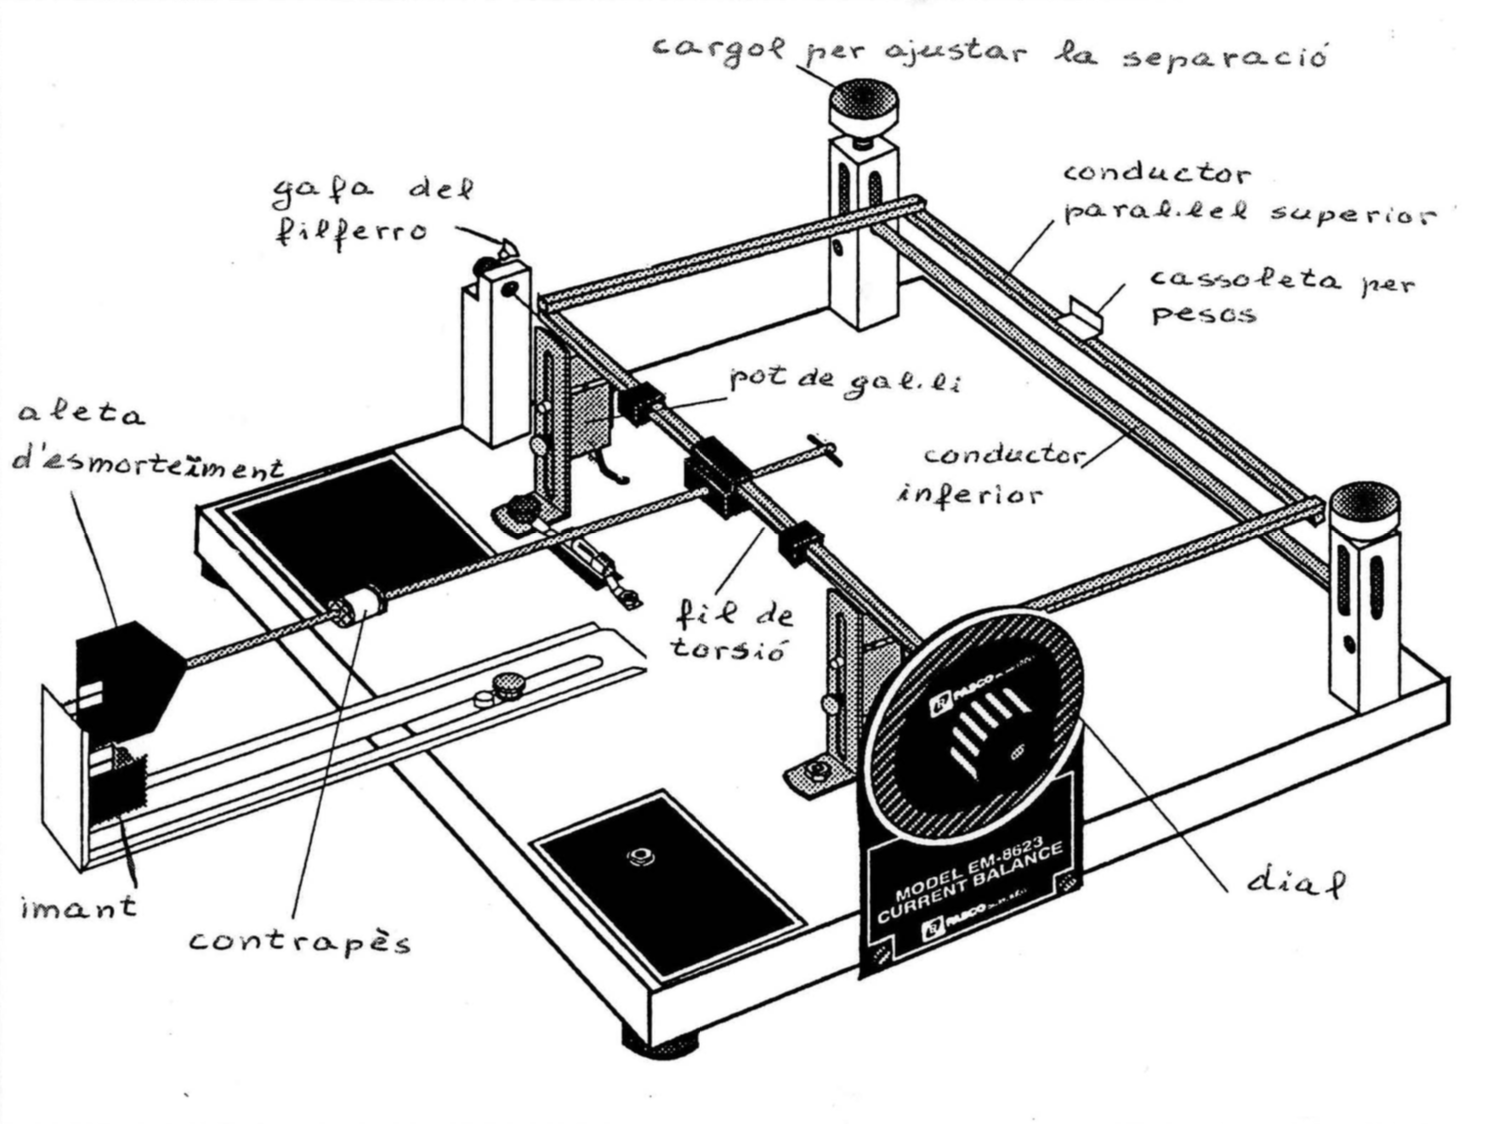
\includegraphics[scale=0.5]{Fig1.png}
	\caption{Muntatge experimental}
	\label{fig:muntatge}
\end{figure}

\section{Resultats i discussió}
El nostre objectiu és representar qualitativament les línies equipotencials produïdes per diferents distribucions de càrrega. Principalment ens centrarem en la forma, però també ens interessa el valor del potencial associat a cada línia, o el valor de la diferència de potencial entre la distribució i la línia, més precisament. En tots els casos, hi fixarem una diferència de potencial de $9V$. Els punts mesurats tenen alguna incertesa associada de $\pm0.02V$, degut a la suma de voltatges. I a més hem realitzat algunes simulacions per a comprovar resultats en tant que forma, però no pas en valors degut a les condicions de contorn. A la \cref{fig:camp carbo} es poden apreciar els papers de carbó ja mencionats i les distribucions de càrrega, acolorides de plata.

\begin{figure}[htb]
  \centering
  % \includegraphics{Foto1.png}
  \caption{Papers de carbó i representacions experimentals}
  \label{fig:camp carbo}
\end{figure}
\subsection{Condensador}
La nostra primera mesura és la dels dos condensadors plano-paral·lels de longitud suposadament infinita i densitat superficial de càrrega uniforme. Fixant una diferència de potencial entre les plaques, vam ser capaços de mesurar diferents línies equipotencials, representades a la \cref{fig:camp condensador}, tant les experimentals com les teòriques.

\begin{figure}[htb]
  \centering
  % \includegraphics{Foto1.png}
  \caption{ Punts experimentals trobats per al condensador, amb les línies experimentals i teòriques.}
  \label{fig:camp condensador}
\end{figure}

Es pot veure que en forma són força semblants, la qual cosa garanteix el bon resultat obtingut. A més, cal afegir que aquest condensador només és infinit a la coordenada $z$, mentre que és finit a la $y$. Per a punts allunyats de la vora, les línies de camp són pràcticament perpendiculars, igual que les aproximacions fetes normalment. Però a la vora hi ha un ràpid creixement i les línies perden el seu caràcter recte.

D'altra banda, d'aquesta distribució pretenem també obtenir una expressió de la capacitat per unitat de longitud. Per a aconseguir-ho, farem ús de l'equació \cref{eq:carrega} per a obtenir una expressió de la càrrega en funció de la longitud de la placa del condensador. Les dades es mostren a la taula, amb les respectives incerteses associades. 

(Fico taula? Hi ha poques dades interessants, gairebé totes són experimentals. La fico a l'annex?)

Cal dir que les distàncies presentaven una incertesa d'origen instrumental de $ \data{}{1}{mm} $, però això es complicava més quan havíem de mesurar $\Delta l_i$, ja que eren línies corbes. Això és una possible font d'error. Per a reduir-la, vam prendre moltes mesures molt properes, de manera que els arcs de corba fossin aproximadament com cordes, és a dir, com rectes. L'incertesa associada a $Q/Z$ combina les incerteses de les altres tres magnituds.

La capacitat promig és llavors $C/\epsilon = \data{1.6}{0.4}{F.m^{-1}}$. Podem calcular també el seu valor teòric, aplicant l'equació \cref{eq:capacitat 2}, i substituint els valors de separació i longitud de les plaques, deixant la permitivitat com a constant desconeguda.
Així s'obté un valor teòric de $C_T/\epsilon = \data{2.0}{0.1}{F.m^{-1}} $. Com podem veure, totes dues mesures són compatibles degut a l'incertesa de l'experimental. També presenten un error relatiu petit, del $20\%$. Sembla llavors una bona estimació.

\subsection{Fils paralels}
La segona distribució de càrrega que vam analitzar va ser la de dos fils o cables infinits. De nou, tenim la secció corresponent a una intersecció amb un pla perpendicular als dos. Idealment només es veurien dos punts de plata, però els fem una mica gruixuts (tots dos amb el mateix radi) per a poder realitzar millor les mesures. Un altre cop vam fixar la diferència de potencial entre els fils i vam procedir a mesurar. Les línies equipotencials i de camp es poden veure a la \cref{fig:camp fils}. Tenim que en forma són molt semblants la teórica i l'experimental.

\begin{figure}[htb]
  \centering
  % \includegraphics{Foto1.png}
  \caption{ Punts experimentals trobats per al condensador, amb les línies experimentals i teòriques.}
  \label{fig:camp fils}
\end{figure}

\subsection{Distribució lliure}
Per a aquesta última distribució tractarem d'avaluar el pes de l'efecte punxa en una distribució tancada per una escorça esfèrica. Observant la \cref{fig:camp carbo}, veiem que la distribució lliure presenta simetria respecte de l'eix $x$. Recordem a més que el mencionat efecte relaciona el camp a la superfície d'un conductor amb el seu radi de curvatura, d'acord amb l'expressió \cref{eq:efecte punxa}, on $E_i$ representa el camp elèctric a la superfície i $r_i$ el radi de curvatura d'aquesta superfície
\begin{equation} \label{eq:efecte punxa}
	E_1r_1=E_2r_2
\end{equation}
de manera que a mesura que el radi decreix, el camp en aquesta part augmenta, esdevenint molt intens en cas que hi hagi punxes.

Per a comprovar aquest efecte, vam provar de dibuixar una figura amb dos radis de curvatura ben diferenciats. Si no existeix l'escorça circular, aquest resultat hauria d'haver-se donat fàcilment, però vam tenir el problema de no ser capaços de preveure l'influència que l'escorça té sobre el camp. Com es pot veure a \todo{Afegir figura del camp lliure}, resulta que el camp és més intens a la zona amb radi de curvatura més gran, i això és justament el contrari del que volíem veure. Notem que superfícies equipotencials més properes implica un canvi més ràpid del mòdul del camp, i per tant, un camp més intens en poca distància.

És complicat realitzar una simulació d'una distribució no coneguda de càrrega. Però això no ens ha d'amoïnar: per a investigacions posteriors una possible millora seria la reducció de les dimensions del cos interior amb respecte de l'escorça esfèrica que l'envolta, o bé aconseguir una millor proporció de les distàncies als extrems del cos interior. Si ens hi fixem, al nostre cas l'extrem de radi menor és a només un centímetre del centre de l'escorça, mentre que l'altre és a quatre centímetres. La solució potser consisteix en col·locar els dos extrems a la mateixa distància, i reduir les dimensions en general.
\section{Conclusions}
\begin{itemize}
	\item Hem obtingut les línies equipotencials generades per un condensador de plaques plano-paral·leles i dos fils infinits també paral·lels. La seva forma és similar a l'obtinguda amb una simulació la qual els calcula a partir de l'expressió analítica.
	\item La capacitat per unitat de longitud del nostre condensador és de $C=(1.6\pm0.4)\epsilon F/m$. Té el mateix ordre de magnitud i un valor molt proper al teòric, entrant aquest dins del marge donat per les incerteses.
	\item No vam poder treure conclusions satisfactòries sobre l'efecte punxa a la distribució lliure. Tot i això, vam trobar una sèrie de canvis que poden ser de gran ajuda en investigacions posteriors, com són la reducció de les dimensions del cos respecte de l'escorça o la millor disposició espaial del cos dins d'aquesta.
\end{itemize}


% Informe 2
\chapter{Força entre corrents} \label{ch:informe 2}
\begin{resum}
	Aquest informe presenta els resultats de l'estudi de la força exercida entre dos corrents para\l.lels pels quals hi circula la mateixa intensitat. Concretament, s'ha provat experimentalment la dependència lineal entre la força i el quadrat de la intensitat i entre la força i l'invers de la distància entre els fils.

	A més, s'ha trobat experimentalment el valor de la constant \( \mu_0 \) a partir de la llei de Biot-Savart, \( \mu_0 = \data{1.25}{0.04e-6}{N.A^{-2}} \) i \( \mu_0 = \data{3.0}{0.4d-6}{N.A^{-2}} \). El primer valor és consistent amb el tabulat, mentre que el segon només n'és de l'ordre. 

	Finalment, s'ha mesurat la component horitzontal del camp magnètic terrestre, obtenint un valor de \( B = \data{1.59}{0.18d-5}{T} \) de l'ordre del que descriuen altres articles.
\end{resum}

\section{Introducció i objectius}
Quan un fil de longitud \( L \) pel qual hi passa un corrent \( I \) és sotmès a un camp magnètic uniforme de mòdul \( B \) experimenta una força proporcional a aquestes tres quantitats i perpendicular tant al fil com al camp magnètic. És a dir
\begin{equation} \label{eq:forca magnetica} 
	F = BIL.
\end{equation}
Per la llei d'Ampère sabem que el camp magnètic a distància \( r \) d'un fil d'aquestes característiques és 
\begin{equation*}
	B = \frac{\mu_0 I}{2\pi r},
\end{equation*}
de manera que deduïm que la força entre dos cables para\l.lels pels quals hi passa corrent en el mateix sentit és atractiva i val
\begin{equation} \label{eq:forca i corrent}
	F = \frac{\mu_0I^2L}{2\pi r}.
\end{equation}

L'objectiu principal d'aquesta pràctica és avaluar experimentalment aquestes relacions. És a dir, s'han fet mesures de la força entre dos fils a diferents corrents i separacions amb l'objectiu d'observar les relacions \( F \propto I^2 \) i \( F \propto r^{-1} \). A més, amb aquestes mesures es pot donar un valor de la constant \( \mu_0 \).  

Finalment també s'ha pogut mesurar el valor de la component radial del camp magnètic terrestre. 

\section{Mètode experimental}
Totes les mesures s'han pres en una balança de corrents. La \cref{fig:balanca} mostra un esquema del dispositiu, amb els elements principals.
\begin{figure}
	\centering
	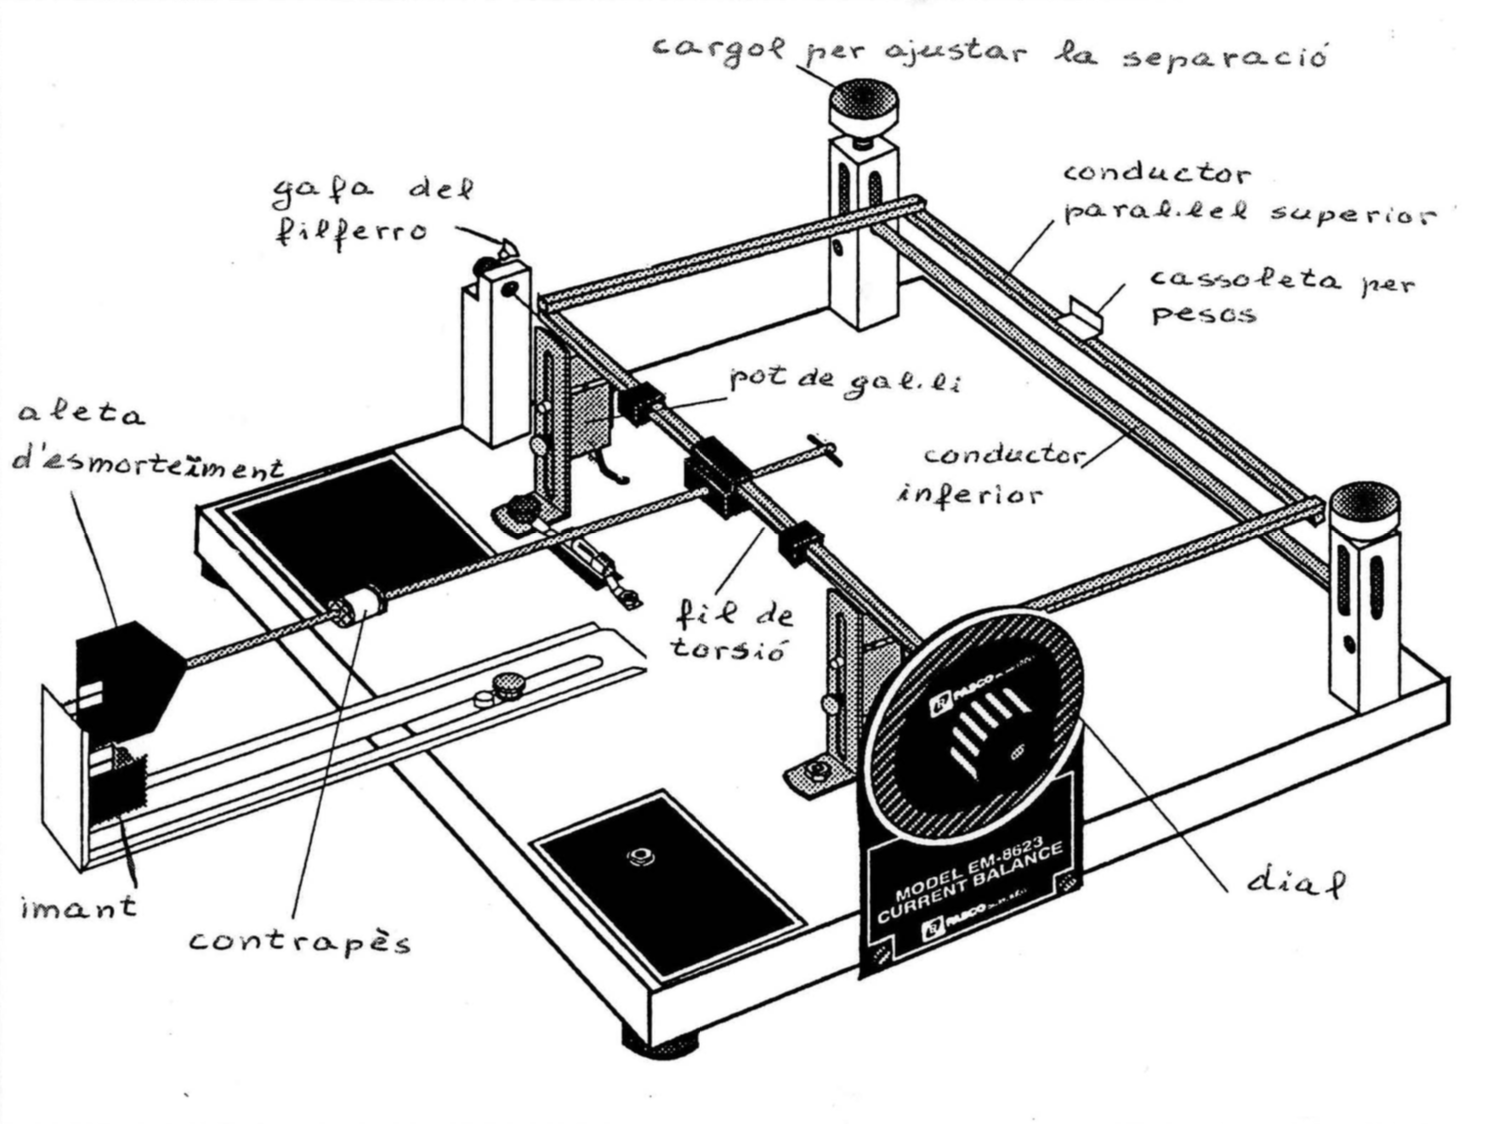
\includegraphics[scale=0.4]{balanca.png}
	\caption{Esquema de la balança de corrents amb els principals elements}
	\label{fig:balanca}
\end{figure}

La balança disposa de dues maneres de determinar la força entre els corrents. Per una banda, disposa d'una cassoleta de pesos on co\l.locar diferents masses. Sabent que, en el moment que la balança es troba equilibrada, la força gravitatòria sobre la massa és igual a la força entre els corrents es pot determinar aquesta última. Per altra banda, la balança també disposa d'un dial i un fil de torsió que poden contrarrestar la força entre els corrents. Sabent que la relació entre els graus que rota el dial i la força que fa és lineal i coneixent la constant de proporcionalitat, es pot determinar també la força entre els corrents.

Cal mencionar que els corrents s'han disposat en direcció nord-sud terrestre per tal que el camp magnètic de la Terra no influís en els resultats.

Cal també comentar que el valor que s'ha pres com a acceleració de la gravetat és \SI{9.80665}{m.s^{-2}} amb incertesa menyspreable en comparació amb la resta d'incerteses que puguin introduir les mesures. S'han pres també sense incertesa els valors de les masses proporcionades al laboratori.

\subsection{Força i intensitat}
Per aquesta part de la pràctica s'ha mesurat la intensitat necessària per compensar la força gravitatòria exercida sobre el cable superior per masses de \SIlist{5; 10; 15; 20; 25}{mg}, un cop havent fixat la distància entre corrents en \SI{8.1}{mm}. Posteriorment s'ha aplicat una regressió lineal entre la força i el quadrat de la intensitat per comprovar la relació predita per l'\cref{eq:forca i corrent}.

\subsection{Força i distància}
En aquesta part, s'ha fixat una intensitat i s'ha anat variant la distància entre els cables. Per cada distància desitjada s'ha determinat la força entre els corrents a partir del mecanisme el fil de torsió. Amb les dades preses s'ha fet una regressió lineal entre la força i l'invers de la distància per verificar la relació predita per l'\cref{eq:forca i corrent} A partir del pendent obtingut en la regressió i l'\cref{eq:forca i corrent} s'ha determinat experimentalment la constant $\mu_0$.

\subsection{Camp magnètic terrestre}
Per aquesta part de l'experiment %Arnau I lof u
s'han orientat els fils en direcció est-oest de manera que fossin perpendiculars al camp magnètic terrestre ---podem, en bona aproximació, suposar que és constant i en la direcció nord-sud---. 

Posteriorment, s'ha fet circular una intensitat fixa només pel fil superior i s'ha determinat la força que patia a través del dial i el fil de torsió. El camp magnètic s'ha determinat a partir de l'\cref{eq:forca magnetica}. 

Com que la força magnètica sobre un fil que porta una intensitat és perpendicular tant al fil com al camp magnètic que la provoca, la disposició de la balança (on els fils es troben sempre horitzontals i només podem mesurar la força veritcal sobre ells) fa impossible la mesura de la component radial del camp magnètic, ja que requeriríem d'un mètode per mesurar la força horitzontal que pateix el fil.

\section{Resultats}
\subsection{Força i intensitat}
La \cref{tab:forca v intensitat} mostra les mitjanes de les intensitats necessàries per contrarrestar la força gravitatòria de les diferents masses usades, essent la distància entre els fils de \SI{8.1}{mm}. La \cref{tab:forca v intensitat (detall)}	de l'annex mostra totes les dades per a cada massa. 

\todo{Si anem curts d'espai el qe primer que treuria són les taules}
\begin{table}[htb]
	\sffamily \small
	\centering
	\caption{Intensitat mitjana necessària per contrarrestar la força gravitatòria de cada massa.}
	\label{tab:forca v intensitat}
	\begin{tabular}{SS[table-parse-only]}
		\toprule
		{Massa (\si{mg})} & {Intensitat (\si{A})} \\
		\midrule
		5  & 2.62 \pm 0.10 \\
		10 & 3.62 \pm 0.18 \\
		15 & 4.49 \pm 0.15 \\
		20 & 5.19 \pm 0.18 \\
		25 & 5.8 \pm 0.3 \\
		\bottomrule
	\end{tabular}
\end{table}

\begin{figure} [htb]
	\centering \small \sffamily
	% GNUPLOT: LaTeX picture with Postscript
\begingroup
\sffamily \small
  \makeatletter
  \providecommand\color[2][]{%
    \GenericError{(gnuplot) \space\space\space\@spaces}{%
      Package color not loaded in conjunction with
      terminal option `colourtext'%
    }{See the gnuplot documentation for explanation.%
    }{Either use 'blacktext' in gnuplot or load the package
      color.sty in LaTeX.}%
    \renewcommand\color[2][]{}%
  }%
  \providecommand\includegraphics[2][]{%
    \GenericError{(gnuplot) \space\space\space\@spaces}{%
      Package graphicx or graphics not loaded%
    }{See the gnuplot documentation for explanation.%
    }{The gnuplot epslatex terminal needs graphicx.sty or graphics.sty.}%
    \renewcommand\includegraphics[2][]{}%
  }%
  \providecommand\rotatebox[2]{#2}%
  \@ifundefined{ifGPcolor}{%
    \newif\ifGPcolor
    \GPcolortrue
  }{}%
  \@ifundefined{ifGPblacktext}{%
    \newif\ifGPblacktext
    \GPblacktextfalse
  }{}%
  % define a \g@addto@macro without @ in the name:
  \let\gplgaddtomacro\g@addto@macro
  % define empty templates for all commands taking text:
  \gdef\gplbacktext{}%
  \gdef\gplfronttext{}%
  \makeatother
  \ifGPblacktext
    % no textcolor at all
    \def\colorrgb#1{}%
    \def\colorgray#1{}%
  \else
    % gray or color?
    \ifGPcolor
      \def\colorrgb#1{\color[rgb]{#1}}%
      \def\colorgray#1{\color[gray]{#1}}%
      \expandafter\def\csname LTw\endcsname{\color{white}}%
      \expandafter\def\csname LTb\endcsname{\color{black}}%
      \expandafter\def\csname LTa\endcsname{\color{black}}%
      \expandafter\def\csname LT0\endcsname{\color[rgb]{1,0,0}}%
      \expandafter\def\csname LT1\endcsname{\color[rgb]{0,1,0}}%
      \expandafter\def\csname LT2\endcsname{\color[rgb]{0,0,1}}%
      \expandafter\def\csname LT3\endcsname{\color[rgb]{1,0,1}}%
      \expandafter\def\csname LT4\endcsname{\color[rgb]{0,1,1}}%
      \expandafter\def\csname LT5\endcsname{\color[rgb]{1,1,0}}%
      \expandafter\def\csname LT6\endcsname{\color[rgb]{0,0,0}}%
      \expandafter\def\csname LT7\endcsname{\color[rgb]{1,0.3,0}}%
      \expandafter\def\csname LT8\endcsname{\color[rgb]{0.5,0.5,0.5}}%
    \else
      % gray
      \def\colorrgb#1{\color{black}}%
      \def\colorgray#1{\color[gray]{#1}}%
      \expandafter\def\csname LTw\endcsname{\color{white}}%
      \expandafter\def\csname LTb\endcsname{\color{black}}%
      \expandafter\def\csname LTa\endcsname{\color{black}}%
      \expandafter\def\csname LT0\endcsname{\color{black}}%
      \expandafter\def\csname LT1\endcsname{\color{black}}%
      \expandafter\def\csname LT2\endcsname{\color{black}}%
      \expandafter\def\csname LT3\endcsname{\color{black}}%
      \expandafter\def\csname LT4\endcsname{\color{black}}%
      \expandafter\def\csname LT5\endcsname{\color{black}}%
      \expandafter\def\csname LT6\endcsname{\color{black}}%
      \expandafter\def\csname LT7\endcsname{\color{black}}%
      \expandafter\def\csname LT8\endcsname{\color{black}}%
    \fi
  \fi
    \setlength{\unitlength}{0.0500bp}%
    \ifx\gptboxheight\undefined%
      \newlength{\gptboxheight}%
      \newlength{\gptboxwidth}%
      \newsavebox{\gptboxtext}%
    \fi%
    \setlength{\fboxrule}{0.5pt}%
    \setlength{\fboxsep}{1pt}%
\begin{picture}(5668.00,3400.00)%
    \gplgaddtomacro\gplbacktext{%
      \csname LTb\endcsname%%
      \put(1078,704){\makebox(0,0)[r]{\strut{}\num{0}}}%
      \put(1078,1117){\makebox(0,0)[r]{\strut{}\num{0.05}}}%
      \put(1078,1529){\makebox(0,0)[r]{\strut{}\num{0.1}}}%
      \put(1078,1942){\makebox(0,0)[r]{\strut{}\num{0.15}}}%
      \put(1078,2354){\makebox(0,0)[r]{\strut{}\num{0.2}}}%
      \put(1078,2767){\makebox(0,0)[r]{\strut{}\num{0.25}}}%
      \put(1078,3179){\makebox(0,0)[r]{\strut{}\num{0.3}}}%
      \put(1210,484){\makebox(0,0){\strut{}\num{5}}}%
      \put(1790,484){\makebox(0,0){\strut{}\num{10}}}%
      \put(2370,484){\makebox(0,0){\strut{}\num{15}}}%
      \put(2950,484){\makebox(0,0){\strut{}\num{20}}}%
      \put(3531,484){\makebox(0,0){\strut{}\num{25}}}%
      \put(4111,484){\makebox(0,0){\strut{}\num{30}}}%
      \put(4691,484){\makebox(0,0){\strut{}\num{35}}}%
      \put(5271,484){\makebox(0,0){\strut{}\num{40}}}%
      \put(4111,1529){\makebox(0,0){\strut{}$r^2$ = \num{0.999}}}%
    }%
    \gplgaddtomacro\gplfronttext{%
      \csname LTb\endcsname%%
      \put(198,1941){\rotatebox{-270}{\makebox(0,0){\strut{}$\mathsf{F \ (\si{mN})}$}}}%
      \put(3240,154){\makebox(0,0){\strut{}$\mathsf{I^2 \ (\si{A})}$}}%
    }%
    \gplbacktext
    \put(0,0){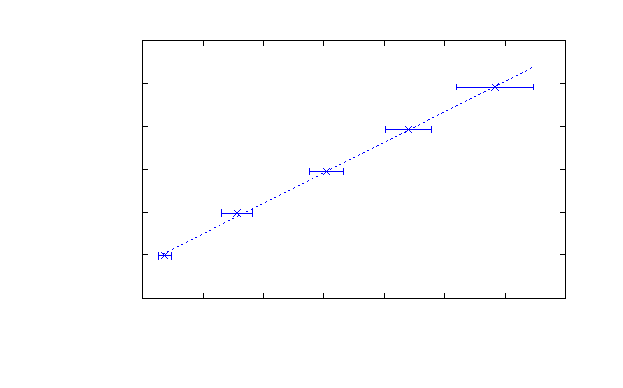
\includegraphics{forca-intensitat}}%
    \gplfronttext
  \end{picture}%
\endgroup

	\caption{Força en funció del quadrat del corrent}
	\label{fig:forca v intensitat}
\end{figure}

Amb els valors presentats a la \cref{tab:forca v intensitat} s'ha fet una regressió lineal entre la força entre corrents i el quadrat de la intensitat, \cref{fig:forca v intensitat}. 

El valor obtingut del pendent de la recta de regressió es de \( \data{7.35}{0.08d-6}{N.A^{-2}} \). A partir d'aquest valor i l'\cref{eq:forca i corrent} s'ha determinat \( \mu_0 = \data{1.25}{0.04d-6}{N.A^{-2}} \) que és compatible amb el valor tabulat, per entrar en el rang d'incerteses i tenir un percentatge d'error petit, del $0.6\%$.

\subsection{Força i distància}
Primerament, a través d'una regressió lineal amb un factor de correlació $r^2=0.985$ s'ha determinat la dependència lineal entre la força exercida pel fil de torsió i la rotació del dial, amb un valor de la constant de proporcionalitat de \( k = \data{3.2}{0.2d-7}{N} \). Les dades de la regressió es poden veure a la \cref{tab:regressio forca-angle} i a la \cref{fig:forca v rotacio}. Així, la força es pot determinar per
\begin{equation} \label{eq:forca i angle}
	F=k\theta
\end{equation}

S'ha fixat una intensitat constant de \( I = \data{5.37}{0.02}{A} \) i s'ha mesurat la rotació necessària del dial per contrarrestrar la força entre corrents. La \cref{tab:forca v desplacament} mostra els resultats. 

\begin{table}[htb]
	\sffamily \small
	\centering
	\caption{Rotació del dial necessària per contrarrestar la força entre corrents a diferents distàncies. La intensitat, fixa, és de \( I = \data{5.37}{0.02}{A} \).}
	\label{tab:forca v desplacament}
	\begin{tabular}{SS}
		\toprule
		{Separació (\data{}{0.001}{m})} &  {Rotació (\data{}{1}{\degree})} \\
		\midrule 
		0.010 & 64 \\ 
		0.009 & 63 \\  
		0.008 & 65 \\  
		0.007 & 87 \\  
		0.006 & 129 \\   
		0.005 & 186 \\   
		\bottomrule
	\end{tabular}
\end{table}

Amb les dades de la \cref{tab:forca v desplacament} s'ha realitzat una regressió lineal entre la força entre corrents, calculada a partir de l'\cref{eq:forca i angle}, i l'invers de la distància, \cref{fig:forca v distancia}.

\begin{figure}[htb]
	\centering
	% GNUPLOT: LaTeX picture with Postscript
\begingroup
\sffamily \small
  \makeatletter
  \providecommand\color[2][]{%
    \GenericError{(gnuplot) \space\space\space\@spaces}{%
      Package color not loaded in conjunction with
      terminal option `colourtext'%
    }{See the gnuplot documentation for explanation.%
    }{Either use 'blacktext' in gnuplot or load the package
      color.sty in LaTeX.}%
    \renewcommand\color[2][]{}%
  }%
  \providecommand\includegraphics[2][]{%
    \GenericError{(gnuplot) \space\space\space\@spaces}{%
      Package graphicx or graphics not loaded%
    }{See the gnuplot documentation for explanation.%
    }{The gnuplot epslatex terminal needs graphicx.sty or graphics.sty.}%
    \renewcommand\includegraphics[2][]{}%
  }%
  \providecommand\rotatebox[2]{#2}%
  \@ifundefined{ifGPcolor}{%
    \newif\ifGPcolor
    \GPcolortrue
  }{}%
  \@ifundefined{ifGPblacktext}{%
    \newif\ifGPblacktext
    \GPblacktextfalse
  }{}%
  % define a \g@addto@macro without @ in the name:
  \let\gplgaddtomacro\g@addto@macro
  % define empty templates for all commands taking text:
  \gdef\gplbacktext{}%
  \gdef\gplfronttext{}%
  \makeatother
  \ifGPblacktext
    % no textcolor at all
    \def\colorrgb#1{}%
    \def\colorgray#1{}%
  \else
    % gray or color?
    \ifGPcolor
      \def\colorrgb#1{\color[rgb]{#1}}%
      \def\colorgray#1{\color[gray]{#1}}%
      \expandafter\def\csname LTw\endcsname{\color{white}}%
      \expandafter\def\csname LTb\endcsname{\color{black}}%
      \expandafter\def\csname LTa\endcsname{\color{black}}%
      \expandafter\def\csname LT0\endcsname{\color[rgb]{1,0,0}}%
      \expandafter\def\csname LT1\endcsname{\color[rgb]{0,1,0}}%
      \expandafter\def\csname LT2\endcsname{\color[rgb]{0,0,1}}%
      \expandafter\def\csname LT3\endcsname{\color[rgb]{1,0,1}}%
      \expandafter\def\csname LT4\endcsname{\color[rgb]{0,1,1}}%
      \expandafter\def\csname LT5\endcsname{\color[rgb]{1,1,0}}%
      \expandafter\def\csname LT6\endcsname{\color[rgb]{0,0,0}}%
      \expandafter\def\csname LT7\endcsname{\color[rgb]{1,0.3,0}}%
      \expandafter\def\csname LT8\endcsname{\color[rgb]{0.5,0.5,0.5}}%
    \else
      % gray
      \def\colorrgb#1{\color{black}}%
      \def\colorgray#1{\color[gray]{#1}}%
      \expandafter\def\csname LTw\endcsname{\color{white}}%
      \expandafter\def\csname LTb\endcsname{\color{black}}%
      \expandafter\def\csname LTa\endcsname{\color{black}}%
      \expandafter\def\csname LT0\endcsname{\color{black}}%
      \expandafter\def\csname LT1\endcsname{\color{black}}%
      \expandafter\def\csname LT2\endcsname{\color{black}}%
      \expandafter\def\csname LT3\endcsname{\color{black}}%
      \expandafter\def\csname LT4\endcsname{\color{black}}%
      \expandafter\def\csname LT5\endcsname{\color{black}}%
      \expandafter\def\csname LT6\endcsname{\color{black}}%
      \expandafter\def\csname LT7\endcsname{\color{black}}%
      \expandafter\def\csname LT8\endcsname{\color{black}}%
    \fi
  \fi
    \setlength{\unitlength}{0.0500bp}%
    \ifx\gptboxheight\undefined%
      \newlength{\gptboxheight}%
      \newlength{\gptboxwidth}%
      \newsavebox{\gptboxtext}%
    \fi%
    \setlength{\fboxrule}{0.5pt}%
    \setlength{\fboxsep}{1pt}%
\begin{picture}(5668.00,3400.00)%
    \gplgaddtomacro\gplbacktext{%
      \csname LTb\endcsname%%
      \put(946,704){\makebox(0,0)[r]{\strut{}\num{0.1}}}%
      \put(946,1117){\makebox(0,0)[r]{\strut{}\num{0.2}}}%
      \put(946,1529){\makebox(0,0)[r]{\strut{}\num{0.3}}}%
      \put(946,1942){\makebox(0,0)[r]{\strut{}\num{0.4}}}%
      \put(946,2354){\makebox(0,0)[r]{\strut{}\num{0.5}}}%
      \put(946,2766){\makebox(0,0)[r]{\strut{}\num{0.6}}}%
      \put(946,3179){\makebox(0,0)[r]{\strut{}\num{0.7}}}%
      \put(1078,484){\makebox(0,0){\strut{}\num{80}}}%
      \put(1677,484){\makebox(0,0){\strut{}\num{100}}}%
      \put(2276,484){\makebox(0,0){\strut{}\num{120}}}%
      \put(2875,484){\makebox(0,0){\strut{}\num{140}}}%
      \put(3474,484){\makebox(0,0){\strut{}\num{160}}}%
      \put(4073,484){\makebox(0,0){\strut{}\num{180}}}%
      \put(4672,484){\makebox(0,0){\strut{}\num{200}}}%
      \put(5271,484){\makebox(0,0){\strut{}\num{220}}}%
    }%
    \gplgaddtomacro\gplfronttext{%
      \csname LTb\endcsname%%
      \put(198,1941){\rotatebox{-270}{\makebox(0,0){\strut{}$\mathsf{F \ (\si{mN})}$}}}%
      \put(3174,154){\makebox(0,0){\strut{}$\mathsf{1/r \ (\si{m^{-1}})}$}}%
    }%
    \gplbacktext
    \put(0,0){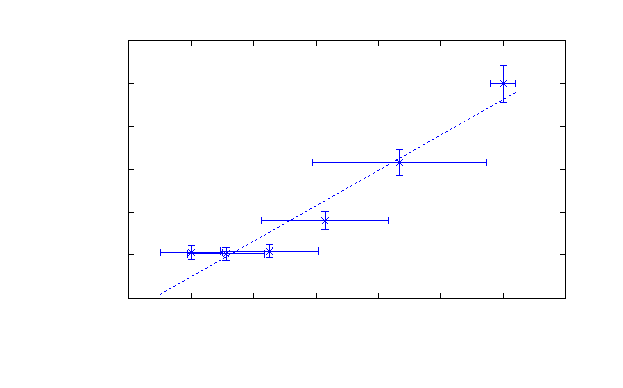
\includegraphics{forca-distancia}}%
    \gplfronttext
  \end{picture}%
\endgroup

	\caption{Força en funció de l'invers de la separació}
	\label{fig:forca v distancia}
\end{figure}

El pendent obtingut a partir de la regressió és \( \data{4.1}{0.6d-6}{N.m} \). A partir d'aquest valor i l'\cref{eq:forca magnetica} s'ha determinat experimentalment el valor de la constant \( \mu_0 = \data{3.0}{0.4d-6}{N.A^{-2}} \). Tenint en compte que el valor teòric de $\mu_0= \SI{1.257e-6}{N.m}$, llavors la mesura té un percentatge d'error del $58\%$. Per tant el resultat no és consistent amb el valor tabulat, possiblement per interferències amb altres elements, però sí de l'orde del valor acceptat.

\subsection{Camp Magnètic Terrestre}
La \cref{tab:camp terrestre} mostra tres mesures d'intensitat i les respectives rotacions del dial per tal de compensar la força que el cable pateix degut a la component radial del camp magnètic terrestre. La força s'obté a partir de l'\cref{eq:forca i angle}, i el camp a partir de l'\cref{eq:forca i corrent}.

\begin{table}[htb]
	\sffamily \small
	\centering
	\caption{Mesures de la component radial del camp magnètic terrestre}
	\label{tab:camp terrestre}
	\begin{tabular}{SSS[table-parse-only]}
		\toprule
		{Intensitat (\data{}{0.01}{A}) } & {Rotació (\data{}{0.01}{\degree}) } & {Camp magnètic (\SI{e-5}{T})} \\
		\midrule
		6.06 & 8& 1.4 \pm 0.3 \\
		6.13 & 8  & 1.4 \pm 0.3 \\
		6.57 & 12 & 2.0 \pm 0.4 \\ 
		\bottomrule
	\end{tabular}
\end{table}

D'aquesta manera, obtenim, a partir de la mitjana aritmètica dels valors de la \cref{tab:camp terrestre}, un valor de la component radial del camp magnètic terrestre de \( B = \data{1.59}{0.18d-5}{T}  \). El resultat no és consistent amb el valor tabulat del camp magnètic a Madrid l'any 1975, possiblement per interferències amb altres elements, però sí que n'és de l'ordre.

\section{Conclusions}
Aquesta experiència s'ha realitzat prenent mesures en una balança de corrents, que permet obtenir la força magnètica que s'exerceixen dos fils para\l.lels suportant intensitats iguals a partir del pes de certes masses o de la rotació d'un dial connectat a un fil de torsió.

Els resultats obtinguts demostren experimentalment la relació lineal entre la força magnètica que s'exerceixen dos fils para\l.lels pels quals hi circula la matreixa intensitat i el quadrat d'aquesta intensitat, així com entre la força i l'invers de la distància entre els fils.

Els experiments també han permès determinar experimentalment la constant $\mu_0$, obtenint valors de \( \mu_0 = \data{1.25}{0.04e-6}{N.A^{-2}} \) i \( \mu_0 = \data{3.0}{0.4d-6}{N.A^{-2}} \). Mentre que el primer és consistent amb el valor tabulat, el segon només n'és de l'ordre. Cal mencionar que la qualitat de la regressió de la \cref{fig:forca v intensitat} és molt millor que la de la \cref{fig:forca v distancia}, i això es veu reflectit en el valor de \( \mu_0 \) obtingut a partir de cada una. 

Finalment, s'ha pogut mesurar la component horitzontal del camp magnètic terrestre, també amb l'ajuda de la balança de corrents, obtenint \( B = \data{1.59}{0.18d-5}{T} \). Aquesta mesura, tot i estar molt possiblement contaminada per soroll i altres efectes del laboratori, és consistent amb l'ordre de magnitud que descriuen altres articles. 


% Informe 3
\chapter{Circuits RLC en sèrie}

\begin{resum}
abstract
\end{resum}

\section{Introducció}
En general, la intensitat que circula per un circuit RLC sotmès a una tensió \( V(t) \) està governada per la següent equació diferencial
\begin{equation} \label{eq:llei RLC}
	\frac{d^2 I}{dt^2} + \frac{R}{L} \frac{dI}{dt} + \frac{1}{LC}I = \frac{1}{L}\frac{dV}{dt},
\end{equation}
on \( R \) és la resistència, \( L \) és la inductància de la bobina i \( C \) la capacitat del condensador. Podem reescriure l'\cref{eq:llei RLC} per trobar la llei que obeeix la tensió que cau a la resistència, \( V_R \):
\begin{equation} \label{eq:llei VR}
	\frac{d^2V_R}{dt^2} + \frac{R}{L}\frac{dV_R}{dt} + \frac{1}{LC}V_R = \frac{R}{L}\frac{dV}{dt}.
\end{equation}
Similarment també podem obtenir la llei que governa la caiguda de tensió en la bobina
\begin{equation} \label{eq:llei VC}
	\frac{d^2V_C}{dt^2} + \frac{R}{L}\frac{dV_C}{dt} + \frac{1}{LC}V_C = \frac{1}{LC}V.
\end{equation}
Observem que totes aquestes equacions són les d'un osci\l.lador forçat. la solució general és la suma d'una solució particular, que rep el nom de terme estacionari, i una solució del sistema homogeni, que rep el nom de terme transitori. La forma del terme transitori depèn dels paràmetres del circuit. En concret depèn del valor del discriminant
\begin{equation*}
	\Delta = \frac{R^2}{L^2} - \frac{4}{LC}.
\end{equation*}
Si \( \Delta < 0 \) el circuit està infraamortit i tenim osci\l.lacions a freqüència 
\begin{equation} \label{eq:freq amortida}
 	\omega = \frac{1}{2}\sqrt{-\Delta} = \frac{1}{2}\sqrt{\frac{4}{LC} - \frac{R^2}{L^2}}. 
\end{equation}
Si \( \Delta > 0 \) aleshores diem que el circuit es troba sobreamortit i no tenim osci\l.lacions, només una caiguda exponencial. En el cas que \( \Delta = 0 \) parlem d'amortiment crític. La resistència que dóna lloca a amortiment crític rep el nom de resistència crítica i es pot calcular imposant \( \Delta = 0 \) i resulta
\begin{equation} \label{eq:resistencia critica}
	R_C = 2\sqrt{\frac{L}{C}}. 
\end{equation}

En tots tres casos, el terme transitori va multiplicat per un factor \( e^{-\lambda t} \) on \( \lambda = \frac{R}{2L} \) rep el nom de constant d'amortiment. Per tant decaurà de forma exponencial, raó per la qual rep el nom de transitori. A la primera part de la pràctica analitzem un circuit en el règim transitori ---i.e. abans de que el terme transitori pugui decaure significativament--- i comprovarem com varia l'amortiment del circuit en funció de \( R \).  

Un cas particularment rellevant és el d'un circuit forçat amb una tensió s'entrada sinusoidal. En aquestes condicions podem observar el fenòment de ressonància, que té lloc quan la tensió d'entrada osci\l.la a la freqüència característica del circuit, 
\begin{equation}\label{eq:freq ressonancia}
	\omega_0 = \frac{1}{\sqrt{LC}}.
\end{equation}
En aquestes condicions ---i en general quan la tensió subministrada osci\l.la sinusoidalment en el temps---, en el règim estacionari totes les magnituds del circuit osci\l.len a la freqüència subministrada \( \omega \). L'amplitud i la diferència de fase d'aquestes osci\l.lacions, però, depenen de \( \omega \). Concretament, per al cas de \( V_R \) es té que el desfasament \( \phi \) amb \( V \) compleix
\begin{equation} \label{eq:desfasament}
	\tan{\phi} = \frac{\frac{1}{C\omega} - L\omega}{R}
\end{equation}
i 
\begin{equation} \label{eq:guany}
	\abs{T_R(\omega)} = \frac{R}{\sqrt{R^2 + \left(L\omega - \frac{1}{C\omega}\right)^2}},
\end{equation}
on \( \abs{T_R(\omega)} \) s'anomena el guany ---\( T_R(\omega) \) és una quantitat complexa que també conté informació sobre el desfasament, però el seu mòdul és precisament el quocient de les amplituds---.

A la segona part de la pràctica analitzarem aquest fenomen en el cas particular de la tensió de la resistència, \( V_R \).   

\section{Mètode experimental}
\subsection{Règim transitori}
\begin{figure}[htb]
	\centering \small \sffamily
	\begin{circuitikz} \draw
	(0,0) to[sqV] (6,0) -- (6,3)
	to[L = \SI{33}{mH}] (4,3)
	to[C = \SI{330}{pF}] (2,3)
	to[vR] (0,3) -- (0,0)
	(2,3) -- (2,4)
	to[voltmeter, l = \( V_C \)] (4,4) -- (4,3)
	;
\end{circuitikz}

	\caption{Esquema del circuit utilitzat per a la primera part}
	\label{fig:esquema transitori}
\end{figure}

En aquesta part de la pràctica s'analitzarà el comportament d'un circuit RLC en el règim transitori. Sobre un circuit amb una bobina d'inductància \( L = \SI{33}{mH} \), una resistència de \( R = \SI{180}{\ohm} \) i un condensador de capacitat \( C  = \SI{330}{pF} \) s'aplicarà un senyal rectangular periòdic d'amplitud \SI{5}{V}. Amb aquests paràmetres podem determinar la resistència crítica \( R_C \) del circuit amb l'\cref{eq:resistencia critica}. El valor de \( R_C \) és \SI{2d4}{\ohm}, de manera que estem en condicions d'infraamortiment. Per a mesurar el període de les osci\l.lacions del voltatge al condensador, \( V_C \), ajustarem la freqüència del senyal rectangular de manera que un període d'aquesta coincideixi amb 10 osci\l.lacions de la tensió al condensador, que s'està mesurant amb un osci\l.loscopi. D'aquesta manera, el període del senyal és 10 vegades el període de les osci\l.lacions.

Per a mesurar la resistència crítica del sistema substituïm la resistència fixa per una de variable. Per a diferents valors de resistència observem comportament infraamortit i sobreamortit. La resistència que es troba a la frontera entre els dos comportaments és \( R_C \).  

\subsection{Règim estacionari}
\begin{figure}[htb]
	\centering \small \sffamily
	\begin{circuitikz} \draw
	(0,0) to[sV] (6,0) -- (6,3)
	to[L = \SI{22}{mH}] (4,3)
	to[C = \SI{15}{mF}] (2,3)
	to[R = \SI{270}{\ohm}] (0,3) -- (0,0)
	(0,3) -- (0,4)
	to[voltmeter, l = \( V_R \)] (2,4) -- (2,3)
	(0,4) -- (0,5.5)
	to[voltmeter, l = \( V \)] (6,5.5) -- (6,3)
	;
\end{circuitikz}

	\caption{Esquema del circuit utilitzat per a la primera part}
	\label{fig:esquema estacionari}
\end{figure}

Per aquesta segona part realitzem mesures sobre un circuit RLC amb capacitat \( C = \SI{15}{mF} \), inductància \( L = \SI{22}{mH} \) i resistència \( R = \SI{2700}{\ohm} \). Després repetirem el procediment amb una resistència de \SI{270}{\ohm}. El circuit estarà sotmès a un voltatge d'entrada \( V \) de freqüència \( \omega \), que es pot controlar a través d'una font. Es mesuraran \( V \) i \( V_r \) amb un osci\l.loscopi.  

En primer lloc es determinarà per a quina freqüència d'entrada el circuit es troba en ressonància ---és a dir, per a quina freqüència el desfasament entre \( V_R \) i \( V \) és nul--- i el valor obtingut es compararà amb el valor calculat per a \( \omega_0 \) segons l'\cref{eq:freq ressonancia}. 

També es determinaran les freqüències de tall, que són les que compleixen \( \abs{T_R(\omega)} = \frac{1}{\sqrt{2}} \). Les freqüències de tall, \( \omega_1 \) i \( \omega_2 \) es poden calcular a priori segons les equacions
\begin{equation} \label{eq:freqs de tall}
	\begin{aligned}
		\omega_1\omega_2 &= \omega_0^2 \\
		\omega_2 - \omega_1 &= \frac{R}{L},
	\end{aligned}
\end{equation}
i els resultats es compararan amb les mesures preses. 

\section{Resultats}
\subsection{Règim transitori}
El valor obtingut per a la freqüència del circuit a partir dels valors coneguts de \( L \), \( C \) i \( R \) i de l'\cref{eq:freq amortida} és \SI{3.03d5}{rad.s^{-1}}. Això dóna un valor per al període de \SI{2.07d-5}{s}. El valor mesurat del període és \data{2.3}{0.1d-5}{s}. Tenim doncs un percentatge d'error de $11\%$. De manera que, tot i que per incerteses els valors no siguin compatibles, són força propers.

Per la resistència crítica, el valor obtingut experimentalment és \data{1.28}{0.01d4}{\ohm}, i el valor obtingut amb l'\cref{eq:resistencia critica} és \SI{2e4}{\ohm}. De nou, el percentatge d'error val $36\%$, resultat no tan satisfactori. 

La mesura del període d'oscil·lació del sistema no és llavors del tot compatible amb el valor teòric. Tampoc ho és el de la resistència crítica. El motiu principal d'aquesta gran discrepància és que en els càlculs no s'han considerat resistències adicionals, a més de la resistència del potenciòmetre. Efectivament, si hom calcula, a partir del valor mesurat del període de l'\cref{eq:freq amortida}, la resistència total a la que està sotmès el circuit, suposant que la capacitat i inductància total es corresponen amb els valors nominals, es troba que la resistència total és d'uns \SI{8.6}{k\ohm}. Com que la mesura es va realitzar amb una resistència nominal de \SI{180}{\ohm}, això vol dir que les resistències desconegudes contribueixen al voltant de \SI{8.4}{k\ohm} a la resistència total. Això vol dir que la resistència crítica del circuit és en realitat de \( \SI{12.8}{k\ohm} + \SI{8.4}{k\ohm} = \SI{21.2}{k\ohm} \), que s'ajusten molt millor als \SI{20}{k\ohm} predits teòricament.  

A la \cref{fig:oscilacions} hi ha representats les tres respostes del circuit: infraamortida, sobreamortida i críticament amortida.

\subsection{Règim estacionari}
Per al circuit amb \( R = \SI{2700}{\ohm} \) la freqüència de ressonància obtinguda experimentalment és \data{8.8}{1}{kHz}. El valor obtingut amb l'\cref{eq:freq ressonancia} és \SI{8.76}{kHz}. La mesura es desvia del valor teòric només en un \SI{0.46}{\percent}. El guany en ressonància és de \SI{98}{\percent}, que es desvia en \SI{2}{\percent} del valor predit. Les freqüències de tall mesurades són \data{3.3}{0.1}{kHz} i \data{24}{1}{kHz} mentre que els valors obtinguts teòricament amb \cref{eq:freqs de tall} són \SI{3.35}{kHz} i \SI{22.9}{kHz}. Les discrepàncies són de \SI{1.5}{\percent} i \SI{4.8}{\percent}.

Per a \( R = \SI{270}{\ohm} \) la freqüència de ressonància és de \data{8.5}{0.2}{kHz}, mentre que el valor teòric és el mateix que per \( R = \SI{2700}{\ohm} \) ja que la freqüència de ressonància només depèn de \( L \) i \( C \). L'error en la mesura és, en aquest cas, del \SI{3}{\percent}.  El guany en ressonància és de \SI{80}{\percent}. Les freqüències de tall mesurades són \data{9.1}{5}{kHz} i \data{7.8}{0.2}{kHz}, mentre que les calculades amb l'\cref{eq:freqs de tall} són \SI{9.79}{kHz} i \SI{7.84}{kHz}. Per tant les desviacions són del \SI{7}{\percent} i del \SI{0.5}{\percent}. 

\begin{figure}[htb]
	\centering \small \sffamily
	% GNUPLOT: LaTeX picture with Postscript
\begingroup
  \makeatletter
  \providecommand\color[2][]{%
    \GenericError{(gnuplot) \space\space\space\@spaces}{%
      Package color not loaded in conjunction with
      terminal option `colourtext'%
    }{See the gnuplot documentation for explanation.%
    }{Either use 'blacktext' in gnuplot or load the package
      color.sty in LaTeX.}%
    \renewcommand\color[2][]{}%
  }%
  \providecommand\includegraphics[2][]{%
    \GenericError{(gnuplot) \space\space\space\@spaces}{%
      Package graphicx or graphics not loaded%
    }{See the gnuplot documentation for explanation.%
    }{The gnuplot epslatex terminal needs graphicx.sty or graphics.sty.}%
    \renewcommand\includegraphics[2][]{}%
  }%
  \providecommand\rotatebox[2]{#2}%
  \@ifundefined{ifGPcolor}{%
    \newif\ifGPcolor
    \GPcolortrue
  }{}%
  \@ifundefined{ifGPblacktext}{%
    \newif\ifGPblacktext
    \GPblacktextfalse
  }{}%
  % define a \g@addto@macro without @ in the name:
  \let\gplgaddtomacro\g@addto@macro
  % define empty templates for all commands taking text:
  \gdef\gplbacktext{}%
  \gdef\gplfronttext{}%
  \makeatother
  \ifGPblacktext
    % no textcolor at all
    \def\colorrgb#1{}%
    \def\colorgray#1{}%
  \else
    % gray or color?
    \ifGPcolor
      \def\colorrgb#1{\color[rgb]{#1}}%
      \def\colorgray#1{\color[gray]{#1}}%
      \expandafter\def\csname LTw\endcsname{\color{white}}%
      \expandafter\def\csname LTb\endcsname{\color{black}}%
      \expandafter\def\csname LTa\endcsname{\color{black}}%
      \expandafter\def\csname LT0\endcsname{\color[rgb]{1,0,0}}%
      \expandafter\def\csname LT1\endcsname{\color[rgb]{0,1,0}}%
      \expandafter\def\csname LT2\endcsname{\color[rgb]{0,0,1}}%
      \expandafter\def\csname LT3\endcsname{\color[rgb]{1,0,1}}%
      \expandafter\def\csname LT4\endcsname{\color[rgb]{0,1,1}}%
      \expandafter\def\csname LT5\endcsname{\color[rgb]{1,1,0}}%
      \expandafter\def\csname LT6\endcsname{\color[rgb]{0,0,0}}%
      \expandafter\def\csname LT7\endcsname{\color[rgb]{1,0.3,0}}%
      \expandafter\def\csname LT8\endcsname{\color[rgb]{0.5,0.5,0.5}}%
    \else
      % gray
      \def\colorrgb#1{\color{black}}%
      \def\colorgray#1{\color[gray]{#1}}%
      \expandafter\def\csname LTw\endcsname{\color{white}}%
      \expandafter\def\csname LTb\endcsname{\color{black}}%
      \expandafter\def\csname LTa\endcsname{\color{black}}%
      \expandafter\def\csname LT0\endcsname{\color{black}}%
      \expandafter\def\csname LT1\endcsname{\color{black}}%
      \expandafter\def\csname LT2\endcsname{\color{black}}%
      \expandafter\def\csname LT3\endcsname{\color{black}}%
      \expandafter\def\csname LT4\endcsname{\color{black}}%
      \expandafter\def\csname LT5\endcsname{\color{black}}%
      \expandafter\def\csname LT6\endcsname{\color{black}}%
      \expandafter\def\csname LT7\endcsname{\color{black}}%
      \expandafter\def\csname LT8\endcsname{\color{black}}%
    \fi
  \fi
    \setlength{\unitlength}{0.0500bp}%
    \ifx\gptboxheight\undefined%
      \newlength{\gptboxheight}%
      \newlength{\gptboxwidth}%
      \newsavebox{\gptboxtext}%
    \fi%
    \setlength{\fboxrule}{0.5pt}%
    \setlength{\fboxsep}{1pt}%
\begin{picture}(5668.00,5668.00)%
    \gplgaddtomacro\gplbacktext{%
      \csname LTb\endcsname%%
      \put(814,704){\makebox(0,0)[r]{\strut{}\num{-5}}}%
      \put(814,2746){\makebox(0,0)[r]{\strut{}\num{0}}}%
      \put(814,4787){\makebox(0,0)[r]{\strut{}\num{5}}}%
      \put(946,484){\makebox(0,0){\strut{}\num{0}}}%
      \put(1811,484){\makebox(0,0){\strut{}\num{20}}}%
      \put(2676,484){\makebox(0,0){\strut{}\num{40}}}%
      \put(3541,484){\makebox(0,0){\strut{}\num{60}}}%
      \put(4406,484){\makebox(0,0){\strut{}\num{80}}}%
      \put(5271,484){\makebox(0,0){\strut{}\num{100}}}%
    }%
    \gplgaddtomacro\gplfronttext{%
      \csname LTb\endcsname%%
      \put(198,2745){\rotatebox{-270}{\makebox(0,0){\strut{}$V_C$ (\si{V})}}}%
      \put(3108,154){\makebox(0,0){\strut{}$t$ (\si{\micro s})}}%
      \csname LTb\endcsname%%
      \put(4001,5495){\makebox(0,0)[r]{\strut{}\footnotesize infraamortiment}}%
      \csname LTb\endcsname%%
      \put(4001,5275){\makebox(0,0)[r]{\strut{}\footnotesize amortiment crític}}%
      \csname LTb\endcsname%%
      \put(4001,5055){\makebox(0,0)[r]{\strut{}\footnotesize sobreamortiment}}%
    }%
    \gplbacktext
    \put(0,0){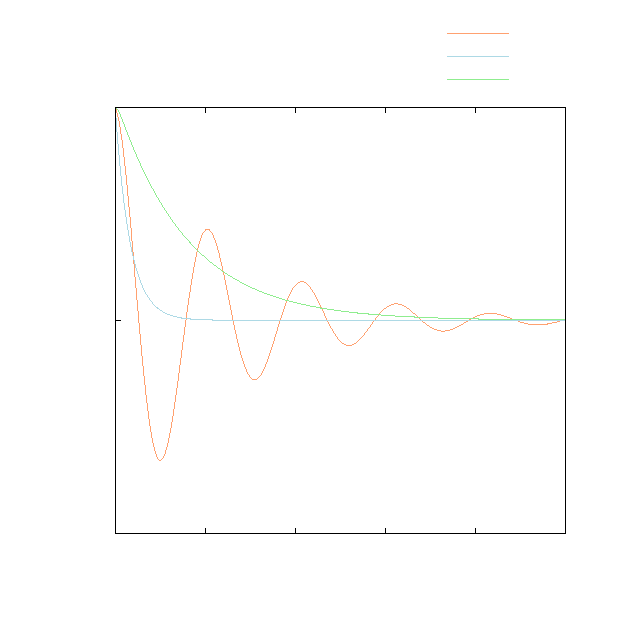
\includegraphics{oscilacions}}%
    \gplfronttext
  \end{picture}%
\endgroup

	\caption{Representació del voltatge al condensador en tres règims d'amortiment diferents}
	\label{fig:oscilacions}
\end{figure}

\section{Conclusions}
\subsection{Règim transitori}



% Informe 4
\chapter{Inductància mútua i transformadors}

\begin{resum}
	L'objectiu d'aquesta pràctica és l'estudi del transformador des d'un punt de vista simplificat i també com a circuit de corrent altern amb una certa impedància. Més concretament, s'estudien els voltatges i les intensitats d'entrada i de sortida del transformador variant la configuració d'aquest, tant amb el circuit secundari en obert com amb una resistència concreta per aquest.
	
	Hem obtingut que la disposició de bobines i ferro que dóna el millor coeficient d'acoblament és aquella que s'assembla més a la forma que segueix el camp d'inducció magnètica d'una bobina. El coeficient, ficant bobines de 400 voltes al primari i al secundari, és del $97\%$. A més hem pogut observar que, a menor nombre de voltes del circuit primari, més gran es torna el flux induït en el secundari. Passa igual amb una intensitat del primari menor.
\end{resum}

\section{Introducció}\label{sec:introducció}

Primerament s'estudiarà el transformador de manera simplificada, tenint en compte que es considera inicialment que tot el flux que genera la primera bobina passa per la segona i a l'inrevés. D'aquesta suposició s'obté la següent relació entre el voltatge d'entrada $V_1$ i el de sortida $V_2$. 

\begin{equation}\label{eq:voltatge transformadors}
  \frac{V_1}{V_2}=\frac{n_1}{n_2}
\end{equation}
On $n_1$ és el nombre de voltes a la bobina del primari i $n_2$ a la del secundari. Per circuits no ideals la suposició anterior obviament no és certa. Això provocarà una certa discrepància entre la situació real i la que descriu l'\cref{eq:voltatge transformadors}. La primera part consistirà bàsicament en l'estudi d'aquesta discrepància per diferents configuracions i bobines.

Seguidament es passara a estudiar el circuit com un circuit amb impedància i, utilitzant les lleis de Kirchhoff, s'obtindran equacions teòriques per descriure la nova situació. L'objectiu d'aquesta segona part serà comprovar de manera experimental la validesa de les equacions teòriques pel transformador connectat a una certa resistència.

\section{Mètode experimental}\label{sec:met}
\subsection{Estudi simplificat}
Per aquesta primera part es tindrà el transformador sense resistències en el secundari com indica la \cref{fig:esquema 1}, evidentment però, s'aniran variant les configuracions del transformador.

\begin{figure}[htb]
  \centering \small \sffamily
  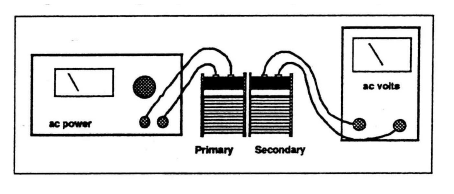
\includegraphics{esquema-transformadors-1.png}
  \caption{Esquema del circuit per l'estudi simplificat}
  \label{fig:esquema 1}
\end{figure}

Com s'explica a la \cref{sec:introducció}, per un transformador real l'\cref{eq:voltatge transformadors} no es compleix. L'expressió que descriu la situació en aquest cas és 
\begin{equation}\label{eq:transformador real}
  k\frac{V_1}{V_2}=\frac{n_1}{n_2}
\end{equation}
on $k$ és el coeficient d'acoblament, un factor que ens parla del grau d'idealitat del transformador, és a dir, és una mesura del flux que indueix el corrent respecte del total. El seu valor es troba entre $0$ i $1$, éssent $k=1$ per al transformador ideal. Per tant, per diferents configuracions del transformador i diferents bobines, s'estudiaran els diferents valors de la constant $k$, fent ús de l'\cref{eq:transformador real}.

\subsection{Estudi com a circuit}\label{sec:metcirc}
En la segona part s'estudia com ja hem dit el transformador com a circuit. Totes les mesures d'aquest apartat són fetes amb el circuit com mostra la figura \cref{fig:esq2}, i com la mateixa figura mostra, en aquest cas, es connecta una resistència al circuit secundari. Per a aquest circuit, emprant les lleis de Kirchh
off s'obtenen certes solucions per les relacions dels voltatges i intensitats d'entrada i sortida. 

\begin{figure}[htbp!]
  \centering \small \sffamily
  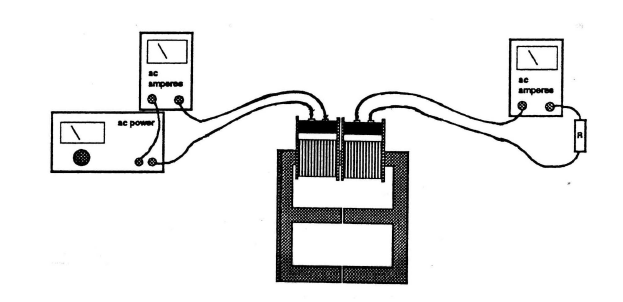
\includegraphics[scale=0.6]{esquema-transformadors-2.png}
  \caption{Esquema del circuit per l'estudi com a circuit amb impedància}
  \label{fig:esq2}
\end{figure}

Inicialment amb una resistència de $R= \SI{1000}{\ohm}$ s'estudien les grans variacions d'intensitat en el circuit primari, només canviant la configuració del transformador. 

Posteriorment, per les bobines de $400$ i $800$ voltes en el primari i amb el circuit obert a la sortida del transformador, es mesura  la intensitat del primari $I_1$, el voltatge del primari $V_1$ i es calcula la reactància $X$ de la bobina segons
\begin{equation}\label{eq:reactancia}
  X=\frac{|V_1|}{|I_1|}.
\end{equation}
L'\cref{eq:reactancia} s'obté de l'aproximació en el cas que la impedància $Z$ compleix que $Z \gg X$. Aquest és el nostre cas ja que al tenir el circuit obert la impedància $Z$ es pot considerar infinita. 

Finalment amb les resistències de \SIlist{1000;100;10}{\ohm}, i amb un voltatge primari de \SI{6}{V}; es mesuren $V_2$, $I_2$ i $I_1$. En els tres casos amb bobines de $400$ voltes, tant al primari com al secundari. Després es repeteix el procediment amb la bobina de $800$ voltes al secundari.

\section{Resultats}
\subsection{Estudi simplificat}
Com s'ha comentat a la \cref{sec:met} s'ha estudiat el comportament de $k$ per cadascuna de les configuracions del transformador de la \cref{fig:configuracions}.
A més, també s'ha estudiat el cas en què no hi havia nucli de ferro a l'interior de les bobines (l'anomenarem $0$). Tot això s'ha fet amb $V_1=\SI{6}{V}$ i amb bobines de $400$ al primari i al secundari.

\begin{figure}[htb]
  \centering \small \sffamily
  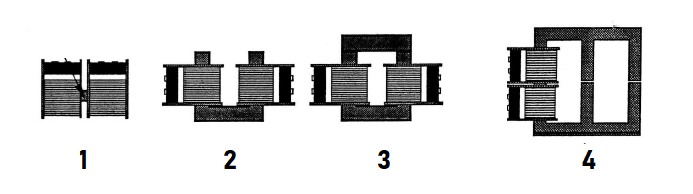
\includegraphics[scale=0.6]{configuracions-transformadors.png}
  \caption{Diferents configuracions del transformador}
  \label{fig:configuracions}
\end{figure}

Així pels cinc casos s'ha obtingut un voltatge de sortida $V_2$ i una $k$. A més, pel cas amb millor voltatge de sortida, s'ha estudiat també la variació de $k$ per les diferents combinacions de bobines.

\begin{table}[htb]
  \centering \small \sffamily
  \caption{Valors del coeficient d'acoblament $k$ i el voltatge secundari $V_2$ per les diferents configuracions}
  \label{tab:acoblament}
	\begin{tabular}{SS[table-parse-only]S[table-parse-only]}
		\toprule
		{Configuració} & { $k$ } & {$V_2$ (\si{V})}  \\
		\midrule
		0 & \data{4.17}{0.17}{\percent} & 0.25 \pm 0.01 \\
		1 & \data{45.13}{0.67}{\percent} & 2.71 \pm 0.04 \\
		2 & \data{35.88}{0.50}{\percent} & 2.15 \pm 0.03 \\
		3 & \data{89.13}{0.83}{\percent} & 5.35 \pm 0.05 \\
		4 & \data{97.46}{0.83}{\percent} & 5.85 \pm 0.05 \\
		\bottomrule
	\end{tabular}
\end{table}

Els resultats comproven que la configuració més eficaç és la número $4$. Els diferents valors de $k$ semblen indicar que hi ha dos fets determinants a l'hora d'augmentar el rendiment del transformador. Primerament el fet que les dues bobines es trobin molt properes l'una a l'altra sembla augmentar considerablement el rendiment, cosa que és lògica d'esperar ja que el flux passarà en més quantitat per la bobina del secundari. A més d'això, el fet que el nucli de ferro segueixi la trajectòria de les línies de camp, també augmenta el rendiment; aquest fet també és d'esperar ja que al ser el ferro un material ferromagnètic condueix bé el flux magnètic a través de l'espai optimitzant-ne l'arribada a l'altra bobina. Evidentment al ser la configuració $4$ la de major potencial de sortida, l'estudi de les diferents bobines ha estat fet amb aquesta.

\begin{table}[htb]
  \centering \footnotesize \sffamily
  \caption{Valors del coeficient d'acoblament $k$ per diferents combinacions de bobines a la configuració 4}
  \label{tab:acoblament 4}
	\begin{tabular}{lS[table-parse-only]S[table-parse-only]S[table-parse-only]S[table-parse-only]S[table-parse-only]}
		\toprule
		& \multicolumn{5}{c}{$N_1$} \\ \cmidrule{2-6}
		{ \( N_2 \) } &200&400&800&1600&3200 \\
		\midrule
		200 &  & \data{96.62}{0.34}{\percent} & \data{95.33}{0.67}{\percent} & \data{94.00}{0.27}{\percent} &  \data{93.93}{0.27}{\percent} \\
		400 & \data{99.58}{0.50}{\percent} & \data{95.60}{0.68}{\percent} & \data{95.58}{0.67}{\percent} & \data{96.33}{0.27}{\percent} & \data{94.17}{0.27}{\percent} \\
		800 & \data{97.81}{0.38}{\percent} & \data{97.08}{0.51}{\percent} & & \data{95.00}{0.67}{\percent} & \data{92.47}{0.33}{\percent} \\ 
		1600 & \data{97.45}{0.16}{\percent} & \data{97.50}{0.34}{\percent} & \data{94.58}{0.33}{\percent} & & \data{92.50}{0.67}{\percent} \\ 
		3200 & \data{98.70}{0.19}{\percent} & \data{97.72}{0.19}{\percent} & \data{94.58}{0.29}{\percent} & \data{95.50}{0.33}{\percent} & \\
		\bottomrule
	\end{tabular}
\end{table}

La \cref{tab:acoblament 4} sembla indicar que, quan més petit sigui el nombre de voltes del circuit primari, millor serà el coeficient d'acoblament. Això té sentit, ja que si veiem que, quan més gran sigui el nombre d'espires, més gran serà el camp creat. Per tant pot ésser més difícil que el camp travessi una superfície donada (la del circuit secundari). És a dir, menor flux del circuit primari implica coeficient d'acoblament major. Això es posa de manifest si ens fixem en la relació entre, per exemple, 800-200 i 200-800.
Tanmateix, les diferències són molt petites i l'estudi no ha estat suficientment exhaustiu com per concloure que la bobina de menor nombre de voltes sempre serà la més eficaç. En efecte, veiem que hi ha anomalíes si posem 200 o 400 voltes al primari. Cal notar que tots els valors són a més molt propers, éssent la diferència més gran de només d'un $5\%$.
\subsection{Estudi com a circuit}
Com s'ha comentat, primerament s'han mesurat les intensitats del primari per diferents configuracions i s'ha analitzat les variacions. Aquestes mesures han estat realitzades amb la bobina de $800$ al primari i la de $400$ al secundari, amb un voltatge primari de \SI{6}{V} i amb una impedància \SI{1000}{\ohm}. 

\begin{table}[htb]
  \centering
  \caption{Valors de intensitat primària $I_1$ i coeficient d'acoblament $k$ per les diferents configuracions}
  \label{tab:I1}
	\begin{tabular}{SS[table-parse-only]S[table-parse-only]}
		\toprule
		{Configuració} & {$k$} & {$I_1$ (\si{A})}  \\
		\midrule
		0 & \data{4.17}{0.17}{\percent} & 0.56 \pm 0.04 \\
		1 & \data{45.13}{0.67}{\percent} & 0.29\pm0.03 \\
		2 & \data{35.88}{0.50}{\percent} & 0.15\pm0.02 \\
		3 & \data{89.13}{0.83}{\percent} & 0.034\pm0.001 \\
		4 & \data{95.58}{0.67}{\percent} & 0.018\pm0.001 \\
		\bottomrule
	\end{tabular}
\end{table}

Amb la informació de la \cref{tab:I1} es veu que $I_1$ varia considerablement amb les diferents configuracions.  Aquesta variació es pot explicar amb la variació de $k$. Per les configuracions amb major $k$ el flux que travessa la bobina secundària augmenta i, per tant, també ho fa el flux de la secundària que travessa la primària. Aquest segon flux crea una força contraelectromotriu que disminueix el voltatge al primari i per tant $I_1$.

Pel que fa a la reactància del circuit, com s'ha comentat a la \cref{sec:metcirc}, es pot calcular la reactància segons l'\cref{eq:reactancia}. Per la bobina de 400 voltes els valors obtinguts han estat $I_{400}= \data{54.33}{0.10}{mA}$ i $X_{400}= \data{110.45}{1.8}{\ohm}$. Per la bobina de 800 voltes els valors han estat $I_{800}= \data{18.55}{0.10}{mA}$ i $X_{800}= \data{323.45}{5.4}{\ohm}$.

Òbviament al tenir menor intensitat la bobina de $800$ voltes, amb el mateix voltatge que la de $400$, això implicarà una major impedància per la de $800$ que és el resultat calculat.

Finalment s'han calculat $I_1$, $I_2$ i $V_2$ per la configuració amb $400$ voltes tant al primari com al secundari, amb les resistències de \SIlist{1000;100;10}{\ohm}.

\begin{table}[htb]
  \centering
  \caption{Valors de $I_1$ i $I_2$ i $V_2$ per \( N \) voltes en el primari i en el secundari}
  \label{tab:400IV}
	\begin{tabular}{cSS[table-parse-only]S[table-parse-only]SSS}
		\toprule
		{$N$} & {$Z$ (\si{\ohm})} & { $I_1$ (\si{mA})} & {$I_2$ (\si{mA})} &  {$V_2$ (\data{}{0.01}{V})} & { $\frac{V_2}{V_1}_{\textsf{exp}}$} & { $\frac{V_2}{V_1}_{\textsf{teo}}$}   \\
		\midrule
		\multirow{3}{*}{400} & 10 & 320 \pm 1 &  325 \pm 1 & 3.46 & 0.58 & 0.69 \\
												 & 100 & 72.2 \pm 0.1 & 42.8 \pm 0.1 & 5.51 & 0.92  & 0.96 \\
												 & 1000 & 51.3 \pm 0.1 & 5.3 \pm 0.1 & 5.76 & 0.96  & 0.96 \\
		\cmidrule{1-1}
		\multirow{3}{*}{800} & 10 & 533 \pm 1 &  248 \pm 1 & 2.68 & 0.45 & 0.32 \\
												 & 100 & 140 \pm 1 & 63.8 \pm 0.1 & 9.37 & 1.59  & 1.94 \\
												 & 1000 & 552 \pm 1 & 10.2 \pm 0.1 & 11.39 & 1.90  & 1.94 \\
		\bottomrule
	\end{tabular}
\end{table}

Per la \cref{tab:400IV} podem veure que, com era d'esperar, a majors impedàncies les intensitats que circulen per ambdós circuits disminueixen. Pel que fa als valors dels guanys aquests són prou propers als valors teòrics, calculant els percentatges d'error surten d'aproximadament el $1\%$, el $4\%$ i el $18\%$ respectivament per les impedàncies de \SIlist{1000;100;10}{\ohm}. Tanmateix hi ha una variació entre els guanys de $Z= \SI{1000}{\ohm}$ i $Z=\SI{100}{\ohm}$ que no hauria d'aparèixer teòricament. Aquest fet probablement és degut a les aproximacions a l'hora de trobar les solucions de les equacions de Kirchhoff pel circuit. El fet que  per $Z= \SI{100}{\ohm}$ $V_2$ disminueixi considerablement, és degut a que el terme de la força contraelectromotriu apareix en l'aproximació de $Z\ll X$ i fa disminuir $V_2$. El fet principal que s'observa relatiu a $Z$, és l'augment del guany per a impedàncies $Z$ més elevades.

En el cas de 800 voltes, els percentatges de error aproximats són de $2\%$, $18\%$ i $38\%$ respectivament per les impedàncies de \SIlist{1000;100;10}{\ohm}, el valor del guany per la resistència de $ \SI{10}{\ohm}$ és la que difereix més notablement del valor teòric esperat. Aquests valors, a més a més, han accentuat en alguns casos els efectes mencionats per la bobina de $400$. Ja que, per exemple, la disminució de $V_2$  per la de $800$ voltes ha estat molt considerable. El valor esperat teòricament era de $V_2=\SI{12}{V}$, en canvi el valor mesurat ha estat de $V_2 = \data{2.68}{0.01}{V}$. També podem observar de la relació entre les dues taules que els valors teòrics han canviat considerablement degut al canvi de $k$. 

\section{Conclusions}
Pel que fa al primer estudi del transformador, les conclusions més interessants han estat veure que sembla que el coeficient d'acoblament, i per tant l'eficiència del circuit, és major per configuracions amb bobines de menys voltes al primari. El nucli de ferro també augmenta en gran mesura $k$, i el fet que aquest segueixi la forma de les línies de camp magnètic també sembla ajudar a augmentar $k$. A més de tots aquests factors, la proximitat de la bobina també sembla ser un factor rellevant, essent més eficients els transformadors amb les bobines més properes.

Per la segona part de l'estudi, s'ha observat que només variant la configuració del transformador ja varia en gran mesura la intensitat de sortida $I_1$. Les configuracions de major $k$ han resultat ser les de menor $I_1$. A més el guany de voltatge $\frac{V_2}{V_1}$ resulta ser major per circuits amb impedàncies $Z$ més elevades. Finalment, també s'ha observat que el voltatge en el circuit secundari disminueix considerablement si la impedància $Z$ del circuit també ho fa.


% Informe 5
\chapter{Mesura de la resistència d'un metall}
\begin{resum}
	L'objectiu d'aquesta pràctica és la mesura experimental de la resistivitat d'un metall. Més concretament, s'ha centrat en la dependència de la resistivitat amb la temperatura. La teoria indica que la resistivitat d'un material, i, en conseqüència, la seva resistència, augmenten linealment amb la temperatura. El nostre experiment, realitzat en un rang de temperatures comprès entre els $\SI{-150}{\celsius}$ i els $\SI{265}{\celsius}$ corrobora aquesta aquesta predicció, ja que la regressió lineal realitzada a partir de les dades de la resistència del metall enfront la temperatura té un coeficient de correlació de $0.997$. S'ha calculat també el factor de proporcionalitat entre la resistència i la temperatura, amb un valor de $\data{0.359}{0.003}{\ohm.\celsius^{-1}}$, i l'ordenada a l'origen, de valor $\data{106.9}{0.4}{\ohm}$.
\end{resum}

\section{Introducció}
En nombrosos conductors, existeix una relació entre el camp elèctric $\vec{E}$ i la densitat de corrent $\vec{J}$ coneguda com la llei d'Ohm, de manera que $\vec{J}=\rho\vec{E}$, on $\rho$ denota la resistivitat del material.

Com que la resistència d'un material de longitud $L$ i secció constant $A$ es pot escriure com $R=\frac{\rho L}{A}$ i la resistivitat augmenta linealment amb la temperatura \( \theta \), en primera aproximació, podem considerar que la resistència d'un material vindrà donada per 
\begin{equation} \label{eq:regressio}
R(\theta)=R_0(1+\beta\theta)
\end{equation}

El nostre objectiu és demostar experimentalment aquesta relació per un material concret i trobar-ne els valors numèrics dels paràmetres $R_0$ i $\beta$.

\section{Mètode experimental}
L'experiment requereix de la mesura de la temperatura del metall i de la seva resistència en diferents moments.

Per tal de mesurar la temperatura es disposa de dos termòmetres de mercuri amb precisió de \SI{1}{\celsius}. Un dels dos s'usa en el rang de temperatures altes ---fins a uns $\SI{300}{\celsius}$--- i l'altre, en el rang de temperatures baixes ---fins a uns $ \SI{-200}{\celsius}$---.

Per tal de mesurar la resistència del material s'ha usat una variació del pont de Wheatstone ---\ref{fig:wheatstone}---, el pont de fil. Com es pot apreciar, el circuit consisteix en quatre resistències connectades en forma de paral·lelogram, tres d'elles conegudes i una desconeguda. Els vèrtex del paral·lelogram s'uneixen amb un amperímetre per tal de mesurar la intensitat que hi circula. El pont estarà equilibrat quan l'amperímetre marqui zero, i llavors podrem trobar la resistència desconeguda a partir de
\begin{equation*}
\frac{R_1}{R_2}=\frac{R_3}{R_4}.
\end{equation*}

\begin{figure}[htb]
	\centering
	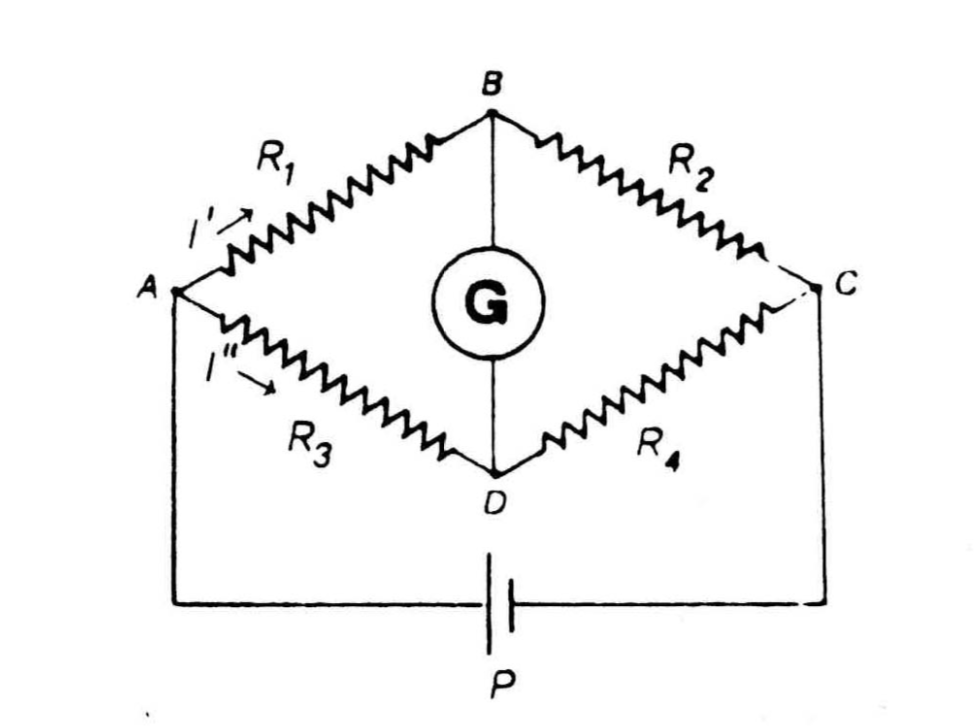
\includegraphics[scale=0.4]{pont.png}
	\caption{Esquema del pont de Wheatstone}
	\label{fig:wheatstone}
\end{figure}

\begin{figure}[htb]
	\centering
	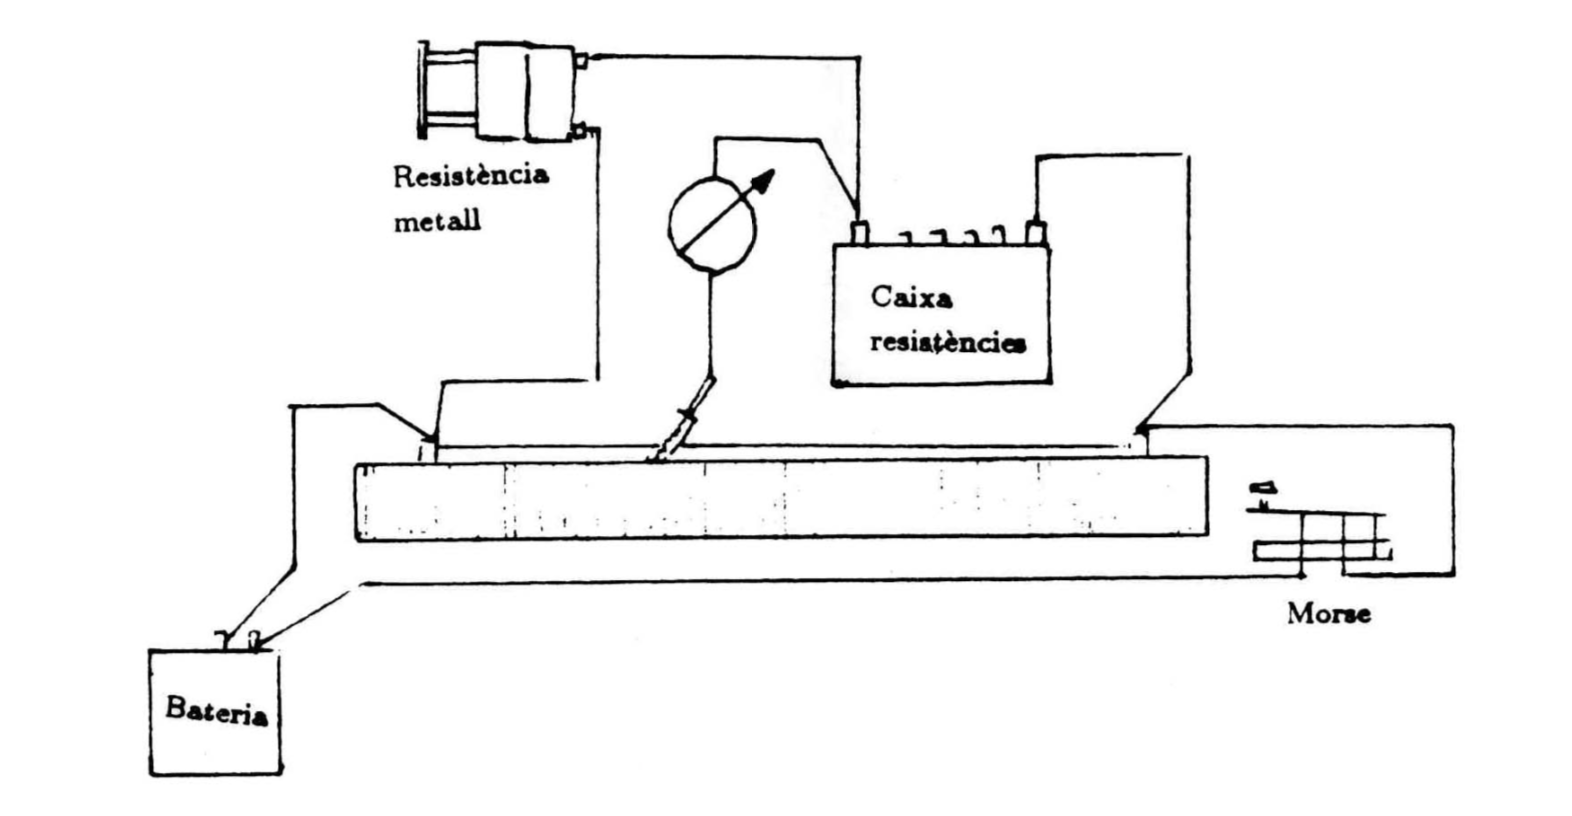
\includegraphics[scale=0.4]{muntatge.png}
	\caption{Esquema del muntatge experimental}
	\label{fig:muntatge resistencia}
\end{figure}

En el pont de fil, dues de les resistències se substitueixen per un fil de longitud coneguda i un cursor que es pot moure per sobre. D'aquesta manera, existeix una relació directa entre el quocient de les longituds i el quocient de les seves resistències. Usant una tercera resistència coneguda, $R_2$, la resistència incògnita, $R_1$, ve donada, quan el pont està equilibrat, per
\begin{equation}\label{eq: <pont>}
R_1=\frac{x}{L-x}R_2
\end{equation}
on $x$ denota la longitud de fil a l'esquerra del cursor i $L$ la longitud total del fil. El muntatge experimental es pot veure a la \cref{fig:muntatge resistencia}. 

Per poder mesurar en el rang d'altes temperatures s'ha escalfat la resistència en un forn. S'ha deixat que la seva temperatura pugés fins a uns $\SI{300}{\celsius}$ i s'han pres les mesures mentre es refredava. Per pendre les mesures en el rang de baixes temperatures, la resistència s'ha submergit en un bany de nitrogen líquid. Un cop extreta del bany, la resistència s'ha mantingut en les proximitats del nitrogen per ralentir-ne el procés d'escalfament i així poder prendre les mesures amb més precisió. 

\section{Resultats}
La \cref{tab:temp i resistencia} mostra la longitud $x$ a l'esquerra del fil a cada temperatura determinada, juntament amb la resistència del metall, usant \ref{eq: <pont>}. La longitud total del fil ha estat fixada en $L=\data{1.000}{0.001}{\meter}$ i la resistència externa en $R_1=\data{100}{1}{\ohm}$.

La regressió lineal amb les dades de la \cref{tab:temp i resistencia} es mostra a la figura \ref{fig:temp v resistencia}. El coeficient de correlació obtingut és de 0.997, el que demostra la linealitat de les dades en l'experiment considerat. S'han obtingut valors de $\data{0.359}{0.003}{\ohm\per\celsius}$ pel pendent i de $\data{106.9}{0.4}{\ohm}$ per l'ordenada a l'origen. Relacionant aquests valors amb l'\cref{eq:regressio} s'obté $R_0=\data{106.9}{0.4}{\ohm}$ i $\beta=\data{336}{3e-5}{\ohm\per\celsius}$.

\begin{figure} [htb]
	\centering
	\small \sffamily
	% % GNUPLOT: LaTeX picture with Postscript
\begingroup
\sffamily \small
  \makeatletter
  \providecommand\color[2][]{%
    \GenericError{(gnuplot) \space\space\space\@spaces}{%
      Package color not loaded in conjunction with
      terminal option `colourtext'%
    }{See the gnuplot documentation for explanation.%
    }{Either use 'blacktext' in gnuplot or load the package
      color.sty in LaTeX.}%
    \renewcommand\color[2][]{}%
  }%
  \providecommand\includegraphics[2][]{%
    \GenericError{(gnuplot) \space\space\space\@spaces}{%
      Package graphicx or graphics not loaded%
    }{See the gnuplot documentation for explanation.%
    }{The gnuplot epslatex terminal needs graphicx.sty or graphics.sty.}%
    \renewcommand\includegraphics[2][]{}%
  }%
  \providecommand\rotatebox[2]{#2}%
  \@ifundefined{ifGPcolor}{%
    \newif\ifGPcolor
    \GPcolortrue
  }{}%
  \@ifundefined{ifGPblacktext}{%
    \newif\ifGPblacktext
    \GPblacktextfalse
  }{}%
  % define a \g@addto@macro without @ in the name:
  \let\gplgaddtomacro\g@addto@macro
  % define empty templates for all commands taking text:
  \gdef\gplbacktext{}%
  \gdef\gplfronttext{}%
  \makeatother
  \ifGPblacktext
    % no textcolor at all
    \def\colorrgb#1{}%
    \def\colorgray#1{}%
  \else
    % gray or color?
    \ifGPcolor
      \def\colorrgb#1{\color[rgb]{#1}}%
      \def\colorgray#1{\color[gray]{#1}}%
      \expandafter\def\csname LTw\endcsname{\color{white}}%
      \expandafter\def\csname LTb\endcsname{\color{black}}%
      \expandafter\def\csname LTa\endcsname{\color{black}}%
      \expandafter\def\csname LT0\endcsname{\color[rgb]{1,0,0}}%
      \expandafter\def\csname LT1\endcsname{\color[rgb]{0,1,0}}%
      \expandafter\def\csname LT2\endcsname{\color[rgb]{0,0,1}}%
      \expandafter\def\csname LT3\endcsname{\color[rgb]{1,0,1}}%
      \expandafter\def\csname LT4\endcsname{\color[rgb]{0,1,1}}%
      \expandafter\def\csname LT5\endcsname{\color[rgb]{1,1,0}}%
      \expandafter\def\csname LT6\endcsname{\color[rgb]{0,0,0}}%
      \expandafter\def\csname LT7\endcsname{\color[rgb]{1,0.3,0}}%
      \expandafter\def\csname LT8\endcsname{\color[rgb]{0.5,0.5,0.5}}%
    \else
      % gray
      \def\colorrgb#1{\color{black}}%
      \def\colorgray#1{\color[gray]{#1}}%
      \expandafter\def\csname LTw\endcsname{\color{white}}%
      \expandafter\def\csname LTb\endcsname{\color{black}}%
      \expandafter\def\csname LTa\endcsname{\color{black}}%
      \expandafter\def\csname LT0\endcsname{\color{black}}%
      \expandafter\def\csname LT1\endcsname{\color{black}}%
      \expandafter\def\csname LT2\endcsname{\color{black}}%
      \expandafter\def\csname LT3\endcsname{\color{black}}%
      \expandafter\def\csname LT4\endcsname{\color{black}}%
      \expandafter\def\csname LT5\endcsname{\color{black}}%
      \expandafter\def\csname LT6\endcsname{\color{black}}%
      \expandafter\def\csname LT7\endcsname{\color{black}}%
      \expandafter\def\csname LT8\endcsname{\color{black}}%
    \fi
  \fi
    \setlength{\unitlength}{0.0500bp}%
    \ifx\gptboxheight\undefined%
      \newlength{\gptboxheight}%
      \newlength{\gptboxwidth}%
      \newsavebox{\gptboxtext}%
    \fi%
    \setlength{\fboxrule}{0.5pt}%
    \setlength{\fboxsep}{1pt}%
\begin{picture}(5668.00,3400.00)%
    \gplgaddtomacro\gplbacktext{%
      \csname LTb\endcsname%%
      \put(1078,704){\makebox(0,0)[r]{\strut{}\num{0}}}%
      \put(1078,1117){\makebox(0,0)[r]{\strut{}\num{0.05}}}%
      \put(1078,1529){\makebox(0,0)[r]{\strut{}\num{0.1}}}%
      \put(1078,1942){\makebox(0,0)[r]{\strut{}\num{0.15}}}%
      \put(1078,2354){\makebox(0,0)[r]{\strut{}\num{0.2}}}%
      \put(1078,2767){\makebox(0,0)[r]{\strut{}\num{0.25}}}%
      \put(1078,3179){\makebox(0,0)[r]{\strut{}\num{0.3}}}%
      \put(1210,484){\makebox(0,0){\strut{}\num{5}}}%
      \put(1790,484){\makebox(0,0){\strut{}\num{10}}}%
      \put(2370,484){\makebox(0,0){\strut{}\num{15}}}%
      \put(2950,484){\makebox(0,0){\strut{}\num{20}}}%
      \put(3531,484){\makebox(0,0){\strut{}\num{25}}}%
      \put(4111,484){\makebox(0,0){\strut{}\num{30}}}%
      \put(4691,484){\makebox(0,0){\strut{}\num{35}}}%
      \put(5271,484){\makebox(0,0){\strut{}\num{40}}}%
      \put(4111,1529){\makebox(0,0){\strut{}$r^2$ = \num{0.999}}}%
    }%
    \gplgaddtomacro\gplfronttext{%
      \csname LTb\endcsname%%
      \put(198,1941){\rotatebox{-270}{\makebox(0,0){\strut{}$\mathsf{F \ (\si{mN})}$}}}%
      \put(3240,154){\makebox(0,0){\strut{}$\mathsf{I^2 \ (\si{A})}$}}%
    }%
    \gplbacktext
    \put(0,0){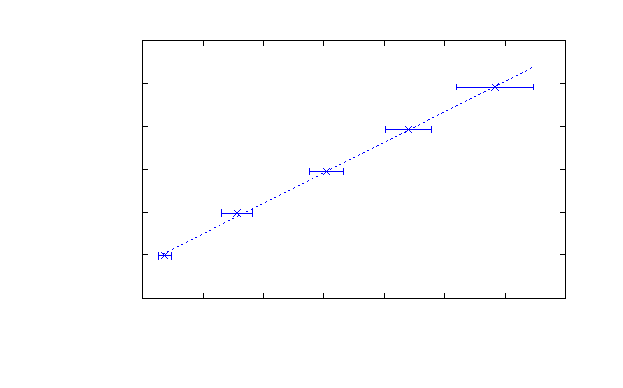
\includegraphics{forca-intensitat}}%
    \gplfronttext
  \end{picture}%
\endgroup

	\caption{Resistència en funció de la temperatura}
	\label{fig:temp v resistencia}
\end{figure}

\section{Conclusions}
S'ha comprovat experimentalment la relació lineal entre la temperatura del metall usat i la seva resistència. El coeficient de correlació, de 0.997, demostra que existeix una relació com la descrita en l'\ref{eq:regressio}. A més, s'han pogut determinar els paràmetres $\beta$ i $R_0$, amb valors de $\data{336}{3e-5}{\per\celsius}$ i $\data{106.9}{0.4}{\ohm}$ respectivament.








\begin{table}[p] 
	\centering \footnotesize \sffamily
	\caption{Mesures experimentals de la resistència a diferents temperatures. El voltatge subministrat és de \data{3.1}{0.2}{V}}
	\label{tab:temp i resistencia}
	\begin{tabular}{SSS}
		\toprule
		{Temperatura (\data{}{1}{\celsius}) } & {Longitud \( x \) (\data{}{0.001}{m})} & {Resistència (\si{\ohm})} \\
		\midrule
		265 & 0.664 & 198 \pm 9 \\
		260 & 0.668 & 201 \pm 9 \\
		255 & 0.665 & 199 \pm 9 \\
		250 & 0.664 & 198 \pm 9 \\
		245 & 0.663 & 197 \pm 9 \\
		240 & 0.661 & 195 \pm 9 \\
		235 & 0.659 & 193 \pm 9 \\
		230 & 0.657 & 192 \pm 9 \\
		225 & 0.655 & 190 \pm 9 \\
		220 & 0.654 & 189 \pm 9 \\
		210 & 0.646 & 182 \pm 8 \\
		200 & 0.643 & 180 \pm 8 \\
		190 & 0.637 & 175 \pm 8 \\
		180 & 0.630 & 170 \pm 8 \\
		170 & 0.627 & 168 \pm 7 \\
		160 & 0.622 & 165 \pm 7 \\
		155 & 0.620 & 163 \pm 7 \\
		150 & 0.616 & 160 \pm 7 \\
		145 & 0.613 & 158 \pm 7 \\
		140 & 0.610 & 156 \pm 7 \\
		135 & 0.608 & 155 \pm 7 \\
		130 & 0.605 & 153 \pm 7 \\
		125 & 0.603 & 152 \pm 7 \\
		120 & 0.600 & 150 \pm 6 \\
		115 & 0.597 & 148 \pm 6 \\
		110 & 0.593 & 146 \pm 6 \\
		105 & 0.585 & 141 \pm 6 \\
		23 & 0.520 & 108 \pm 5 \\
		-20 & 0.485 & 94 \pm 4{}\\
		-25 & 0.484 & 94 \pm 4 \\
		-30 & 0.481 & 93 \pm 4 \\
		-35 & 0.478 & 92 \pm 4 \\
		-40 & 0.474 & 90 \pm 4 \\
		-45 & 0.470 & 88 \pm 4 \\
		-49 & 0.468 & 88 \pm 4 \\
		-55 & 0.464 & 87 \pm 4 \\
		-60 & 0.459 & 85 \pm 4 \\
		-65 & 0.457 & 84 \pm 4 \\
		-70 & 0.452 & 82 \pm 3 \\
		-75 & 0.447 & 81 \pm 3 \\
		-80 & 0.445 & 80 \pm 3 \\
		-85 & 0.441 & 79 \pm 3 \\
		-90 & 0.436 & 77 \pm 3 \\
		-95 & 0.431 & 76 \pm 3 \\
		-100 & 0.424 & 74 \pm 3 \\
		-105 & 0.417 & 72 \pm 3 \\
		-110 & 0.409 & 69 \pm 3 \\
		-115 & 0.398 & 66 \pm 3 \\
		-150 & 0.365 & 57 \pm 3 \\
		\bottomrule
	\end{tabular}
\end{table}  


% Informe 7
\chapter{Camps magnètics d'espires i bobines}
\begin{resum}
Aquesta pràctica té com a objectiu principal l'estudi dels camps magnètics creats per diferents configuracions d'espires i bobines. Mitjançant una sonda Hall s'han mesurat els camps creats, al seu centre, per espires de radis diferents, així com per conjunts de una, dues i tres espires. De la mateixa manera s'han realitzat mesures del camp magnètic al llarg de l'eix de bobinas de diversos radis.

Amb les dades experimentals s'ha posat a prova la dependència del camp magnètic d'una espira del seu radi i també del nombre d'espires, tal i com prediu la llei de Biot-Savart. També s'ha pogut trobar un valor per a la permeabilitat magnètica del buit, \( \mu_0 \).
\end{resum}
\todo{error relatiu comès}

\section{Introducció}
En la primera part de la pràctica s'estudiarà el camp magnètic degut a conjunts d'espires. Si considerem un conjunt de \( N \) espires de radi \( R \) per les que hi circula un corrent constant \( I \), un càlcul elemental amb la llei de Biot-Savart ens dóna que el camp magnètic \( \vec{B} \) al seu centre és
\begin{equation}\label{eq:camp espira}
  \vec{B}=\frac{\mu_0 I N}{2 R}\vec{e}_z,
\end{equation}
on \( \vec{e}_z \) és el vector unitari perpendicular al pla de les espires. Així doncs esperem poder observar les relacions \( B \propto R^{-1} \) i \( B \propto N \). 

Pel que fa al camp magnètic d'una bobina, sabem que en el cas d'una bobina infinita el camp en el seu interior és constant i nul a l'exterior. En el cas d'una bobina finita de longitud \( L \), radi \( R \), \( N \) voltes i per la qual hi passa una intensitat constant \( I \), el camp a punts del seu eix es pot trobar de manera exacta mitjançant la llei de Biot-Savart i resulta
\begin{equation}\label{eq:camp bobina}
  \vec{B}=\frac{\mu_0 I N}{2 L}\left(\frac{z + L/2}{\sqrt{R^2+(z+L/2)^2}} - \frac{z - L/2}{\sqrt{R^2 + (z - L/2)^2}}\right) \vec{e}_z,
\end{equation}
on \( z \) és la posició de la sonda al llarg de l'eix de la bobina ---fixant \( z = 0 \) al seu centre--- i \( \vec{e}_z \) és el vector unitari para\l.lel a l'eix. Quan \( L \gg R \) aleshores l'\cref{eq:camp bobina} dóna lloc a un camp que és gairebé constant per \( \abs{z} < L/2 \) i que decau molt depressa cap a 0 quan \( \abs{z} > L/2 \). 

\section{Mètode experimental}
\subsection{Espires}
Per a realitzar les mesures s'ha fet servir la disposició que es mostra a la \cref{fig:circuit teslametre}. Les espires i la sonda estaven cada una sobre un suport de manera que la sonda estigués a la mateixa alçada que el centre de l'espira. La sonda també estava muntada sobre una rail de manera que es mantingués sempre sobre l'eix perpendicular de les espires.

\begin{figure}[htb]
  \centering \small \sffamily
  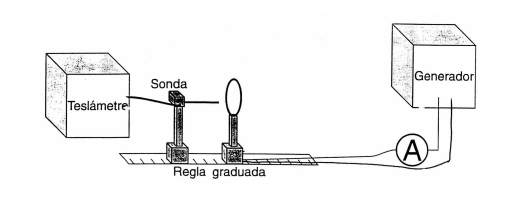
\includegraphics{circuit-teslametre.png}
  \caption{Esquema del circuit emprat per a mesurar el camp magnètic}
  \label{fig:circuit teslametre}
\end{figure}

El corrent subministrat per la font es va fixar a \SI{4.00}{A} i tot seguit la sonda es va desplaçar fins al centre de l'espira ---de la qual ja s'havia mesurat el radi---. Cal mencionar que el sensor de camp magnètic no es troba exactament a la punta de la sonda, de manera que és complicat determinar exactament quan és que efectivament s'estava mesurant el camp al centre. Com que, d'acord amb el resultat teòric, el camp magnètic s'una espira és màxim al seu centre, es va considerar el màxim valor registrat pel teslàmetre. Degut a la seva alta sensibilitat, el teslàmetre trigava un temps considerable a estabilitzar la seva lectura després de canvis bruscos en el camp magnètic. 

S'han pres sis mesures del camp per a cada espira---tres en total, cada una amb un radi diferent. Tres amb un sentit del corrent i tres amb el corrent en sentit oposat. Aleshores s'ha fet el promig de les sis lectures per a minimitzar errors aleatoris deguts a fluctuacions en la mesura del teslàmetre.   

Posteriorment s'ha mesurat el camp al centre del conjunt de 1, 2 i 3 espires seguint el mateix procediment.

\subsection{Bobines}
Per la mesura del camp a l'interior de les bobines s'ha fet servir el mateix circuit que es mostra a la \cref{fig:circuit teslametre}.

Ajustant la intensitat a \data{1.00}{0.01}{A} a l'amperímetre, s'ha mesurat el camp a diversos punts a l'interior de la bobina. Per fer-ho s'ha ajustat l'alçada de la sonda de manera que aquesta quedi sobre l'eix de la bobina. Començant pel punt immediatament a l'exterior de la bobina s'ha fet avançar la sonda sobre el regle mesurant el camp cada \SI{3}{cm} de manera que n'han resultat 8 mesures a diferents punts de l'eix.

Aquest mateix procediment s'ha repetit per cada una de les bobines diferents.  

\section{Resultats}
\subsection{Espires}\label{sec:espires}
Com s'ha mencionat anteriorment, en aquesta secció es presenten els resultats relatius a la part de la pràctica referent a les espires. A la \cref{tab:camp espires en funcio de r} es presenten les mesures del camp magnètic al centre d'una espira en funció del seu radi. 

\begin{table}[htb]
  \centering \small \sffamily
  \caption{Taula de valors teòrics i experimentals}
  \label{tab:camp espires en funcio de r}
	\begin{tabular}{SSS}
		\toprule
		{Radi (\data{}{0.2}{cm})} & { \( B_{\textsf{exp}}\ (\SI{d-5}{T}) \) } & { \( B_{\textsf{teò}}\ (\SI{d-5}{T}) \) } \\
		\midrule
		3.0 & 7.3\pm1.4 & 8.4\pm0.4 \\
		4.3 & 6.0\pm1.6 & 5.9\pm0.2 \\
		6.0 & 5.0\pm1.6 & 4.2\pm0.1 \\
		\bottomrule
	\end{tabular}
\end{table}

Les incerteses dels camps experimentals de la \cref{tab:camp espires en funcio de r} han estat calculades segons la desviació estàndard de les diferents mesures realitzades. Pel que fa a les incerteses teòriques, aquestes han estat calculades per propagació d'incerteses de la fórmula \cref{eq:camp espira}. Com podem veure en els tres casos, els valors experimentals amb els seus respectius intervals d'incertesa coincideixen en alguns punts amb els valors teòrics i els seus intervals, per tant els resultats són compatibles. Es pot observar que l'incertesa dels resultats experimentals és considerablement major. Això és degut a les imprecisions dels aparells emprats per a la mesura dels camps, especialment a les contínues fluctuacions del teslàmetre. 

Tanmateix, el fet més rellevant que podem observar és la disminució del camp a l'interior de l'espira a mesura que augmenta el seu radi. Aquest resultat ja era el que esperavem teòricament. Per fer més èmfasi en aquest fet es presenta la gràfica de lacref{fig:camp espira}, on es representa el camp magnètic al centre en funció del radi de l'espira.
\begin{figure}[htb]
  \centering
  % 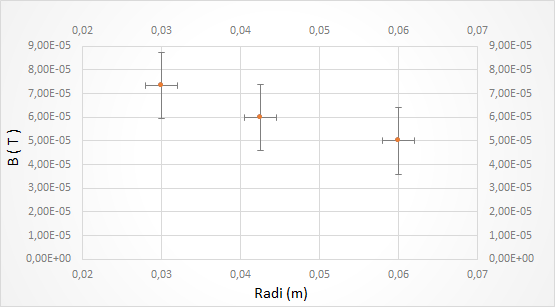
\includegraphics[width=100mm]{graf1.png}
  \caption{Camp magnètic al centre en funció del radi de l'espira}
  \label{fig:camp espira}
\end{figure}

Com es comentava, s'observa que el camp a l'interior es va  atenuant a mesura que s'augmenta el radi de l'espira. Tot i que és difícil d'apreciar ja que només s'ha fet la mesura amb tres radis diferents, es pot comprovar numèricament que el camp magnètic decau com \( \frac{1}{R} \). Aquesta és per tant la forma de funció que observaríem si es tinguessin valors infinits de radis d'espires i els seus camps respectius.

La taula \cref{tab:camp espires en funcio de n} presenta els camp magnètics teòrics i experimentals al centre dels conjunts de 1, 2 i 3 espires. 

\begin{table}[htb]
	\centering \small \sffamily
	\caption{Valors teòrics i experimentals del camp magnètic al centre d'un conjunt de \( N \) espires}
	\label{tab:camp espires en funcio de n}
	\begin{tabular}{SSS}
		\toprule
		{Nombre d'espires \( N \)} & { \( B_{\textsf{exp}}\ (\SI{d-5}{T}) \) } & { \( B_{\textsf{teò}}\ (\SI{d-5}{T}) \) } \\
		\midrule
		1 & 5.0\pm1.6 & 4.2\pm0.1 \\
		2 & 8.8\pm1.5 & 8.4\pm0.2 \\
		3 & 12.3\pm1.5 & 12.6\pm0.3 \\
		\bottomrule
	\end{tabular}
\end{table}

Podem observar que en aquest cas els intervals dels camps teòrics i experimentals també se solapen i per tant les observacions satisfan l'esperat. Altra vegada tornem a tenir incerteses majors pels valors experimentals pel mateix fet anteriorment mencionat. Els resultats ens permeten observar que com més espires introduïm al conjunt més intens es torna el camp al centre d'aquest. Aquesta dependència es pot observar clarament al gràfic experimental del camp al centre en funció del nombre d'espires que s'exposa a la \cref{fig:camp vs n}.

\begin{figure}[htb]
  \centering
  % 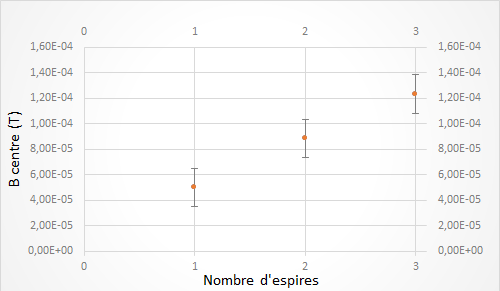
\includegraphics[width=100mm]{graf2.png}
  \caption{Camp al centre en funció del nombre d'espires}
  \label{fig:camp vs n}
\end{figure}

Podem veure a la regressió de la \cref{fig:camp vs n} que aquesta dependència és lineal com s'esperava dels valors teòrics obtinguts a partir de la \cref{eq:camp espira}. El valor de $\mu_{0}$ obtingut a partir de la regressió tenint en compte que el pendent segons \cref{eq:camp espira} és $\frac{\mu_{0}I}{2R}$  s'obté un valor de $\mu_{0} = \data{1.10}{0.37d-6}{N.A^{-2}} $ que és compatible amb el valor teòric de $\mu_{0}\approx \SI{1.26d-6}{N.A^{-2}} $. Així doncs, vist que el camp augmenta de manera directament proporcional al nombre d'espires, els resultats d'aquest apartat queden interpretats.

\subsection{Bobines}\label{sec:bobines}
\begin{figure}[tp]
	\sffamily \small
	\centering
	% GNUPLOT: LaTeX picture with Postscript
\begingroup
\sffamily \small
  \makeatletter
  \providecommand\color[2][]{%
    \GenericError{(gnuplot) \space\space\space\@spaces}{%
      Package color not loaded in conjunction with
      terminal option `colourtext'%
    }{See the gnuplot documentation for explanation.%
    }{Either use 'blacktext' in gnuplot or load the package
      color.sty in LaTeX.}%
    \renewcommand\color[2][]{}%
  }%
  \providecommand\includegraphics[2][]{%
    \GenericError{(gnuplot) \space\space\space\@spaces}{%
      Package graphicx or graphics not loaded%
    }{See the gnuplot documentation for explanation.%
    }{The gnuplot epslatex terminal needs graphicx.sty or graphics.sty.}%
    \renewcommand\includegraphics[2][]{}%
  }%
  \providecommand\rotatebox[2]{#2}%
  \@ifundefined{ifGPcolor}{%
    \newif\ifGPcolor
    \GPcolortrue
  }{}%
  \@ifundefined{ifGPblacktext}{%
    \newif\ifGPblacktext
    \GPblacktextfalse
  }{}%
  % define a \g@addto@macro without @ in the name:
  \let\gplgaddtomacro\g@addto@macro
  % define empty templates for all commands taking text:
  \gdef\gplbacktext{}%
  \gdef\gplfronttext{}%
  \makeatother
  \ifGPblacktext
    % no textcolor at all
    \def\colorrgb#1{}%
    \def\colorgray#1{}%
  \else
    % gray or color?
    \ifGPcolor
      \def\colorrgb#1{\color[rgb]{#1}}%
      \def\colorgray#1{\color[gray]{#1}}%
      \expandafter\def\csname LTw\endcsname{\color{white}}%
      \expandafter\def\csname LTb\endcsname{\color{black}}%
      \expandafter\def\csname LTa\endcsname{\color{black}}%
      \expandafter\def\csname LT0\endcsname{\color[rgb]{1,0,0}}%
      \expandafter\def\csname LT1\endcsname{\color[rgb]{0,1,0}}%
      \expandafter\def\csname LT2\endcsname{\color[rgb]{0,0,1}}%
      \expandafter\def\csname LT3\endcsname{\color[rgb]{1,0,1}}%
      \expandafter\def\csname LT4\endcsname{\color[rgb]{0,1,1}}%
      \expandafter\def\csname LT5\endcsname{\color[rgb]{1,1,0}}%
      \expandafter\def\csname LT6\endcsname{\color[rgb]{0,0,0}}%
      \expandafter\def\csname LT7\endcsname{\color[rgb]{1,0.3,0}}%
      \expandafter\def\csname LT8\endcsname{\color[rgb]{0.5,0.5,0.5}}%
    \else
      % gray
      \def\colorrgb#1{\color{black}}%
      \def\colorgray#1{\color[gray]{#1}}%
      \expandafter\def\csname LTw\endcsname{\color{white}}%
      \expandafter\def\csname LTb\endcsname{\color{black}}%
      \expandafter\def\csname LTa\endcsname{\color{black}}%
      \expandafter\def\csname LT0\endcsname{\color{black}}%
      \expandafter\def\csname LT1\endcsname{\color{black}}%
      \expandafter\def\csname LT2\endcsname{\color{black}}%
      \expandafter\def\csname LT3\endcsname{\color{black}}%
      \expandafter\def\csname LT4\endcsname{\color{black}}%
      \expandafter\def\csname LT5\endcsname{\color{black}}%
      \expandafter\def\csname LT6\endcsname{\color{black}}%
      \expandafter\def\csname LT7\endcsname{\color{black}}%
      \expandafter\def\csname LT8\endcsname{\color{black}}%
    \fi
  \fi
    \setlength{\unitlength}{0.0500bp}%
    \ifx\gptboxheight\undefined%
      \newlength{\gptboxheight}%
      \newlength{\gptboxwidth}%
      \newsavebox{\gptboxtext}%
    \fi%
    \setlength{\fboxrule}{0.5pt}%
    \setlength{\fboxsep}{1pt}%
\begin{picture}(5668.00,3400.00)%
    \gplgaddtomacro\gplbacktext{%
      \csname LTb\endcsname%%
      \put(946,704){\makebox(0,0)[r]{\strut{}\num{0}}}%
      \put(946,1117){\makebox(0,0)[r]{\strut{}\num{0.5}}}%
      \put(946,1529){\makebox(0,0)[r]{\strut{}\num{1}}}%
      \put(946,1942){\makebox(0,0)[r]{\strut{}\num{1.5}}}%
      \put(946,2354){\makebox(0,0)[r]{\strut{}\num{2}}}%
      \put(946,2767){\makebox(0,0)[r]{\strut{}\num{2.5}}}%
      \put(946,3179){\makebox(0,0)[r]{\strut{}\num{3}}}%
      \put(1078,484){\makebox(0,0){\strut{}\num{-15}}}%
      \put(1777,484){\makebox(0,0){\strut{}\num{-10}}}%
      \put(2476,484){\makebox(0,0){\strut{}\num{-5}}}%
      \put(3175,484){\makebox(0,0){\strut{}\num{0}}}%
      \put(3873,484){\makebox(0,0){\strut{}\num{5}}}%
      \put(4572,484){\makebox(0,0){\strut{}\num{10}}}%
      \put(5271,484){\makebox(0,0){\strut{}\num{15}}}%
    }%
    \gplgaddtomacro\gplfronttext{%
      \csname LTb\endcsname%%
      \put(198,1941){\rotatebox{-270}{\makebox(0,0){\strut{}$\mathsf{B \ (\si{mT})}$}}}%
      \put(3174,154){\makebox(0,0){\strut{}$\mathsf{z \ (\si{cm})}$}}%
    }%
    \gplbacktext
    \put(0,0){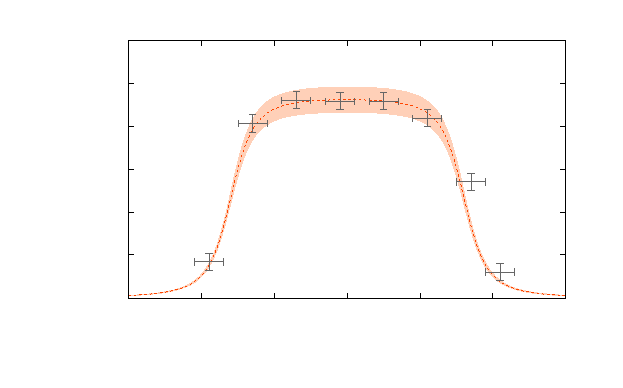
\includegraphics{camp-300-33}}%
    \gplfronttext
  \end{picture}%
\endgroup

	\caption{Camp magnètic al llarg de l'eix d'una bobina de 300 voltes, longitud \SI{16}{cm} i diàmetre \SI{3.3}{cm} per la que hi passa un corrent constant de \SI{1}{A}.}
	\label{fig:camp 300/33}
\end{figure}

\begin{figure}[tp]
	\sffamily \small
	\centering
	% GNUPLOT: LaTeX picture with Postscript
\begingroup
\sffamily \small
  \makeatletter
  \providecommand\color[2][]{%
    \GenericError{(gnuplot) \space\space\space\@spaces}{%
      Package color not loaded in conjunction with
      terminal option `colourtext'%
    }{See the gnuplot documentation for explanation.%
    }{Either use 'blacktext' in gnuplot or load the package
      color.sty in LaTeX.}%
    \renewcommand\color[2][]{}%
  }%
  \providecommand\includegraphics[2][]{%
    \GenericError{(gnuplot) \space\space\space\@spaces}{%
      Package graphicx or graphics not loaded%
    }{See the gnuplot documentation for explanation.%
    }{The gnuplot epslatex terminal needs graphicx.sty or graphics.sty.}%
    \renewcommand\includegraphics[2][]{}%
  }%
  \providecommand\rotatebox[2]{#2}%
  \@ifundefined{ifGPcolor}{%
    \newif\ifGPcolor
    \GPcolortrue
  }{}%
  \@ifundefined{ifGPblacktext}{%
    \newif\ifGPblacktext
    \GPblacktextfalse
  }{}%
  % define a \g@addto@macro without @ in the name:
  \let\gplgaddtomacro\g@addto@macro
  % define empty templates for all commands taking text:
  \gdef\gplbacktext{}%
  \gdef\gplfronttext{}%
  \makeatother
  \ifGPblacktext
    % no textcolor at all
    \def\colorrgb#1{}%
    \def\colorgray#1{}%
  \else
    % gray or color?
    \ifGPcolor
      \def\colorrgb#1{\color[rgb]{#1}}%
      \def\colorgray#1{\color[gray]{#1}}%
      \expandafter\def\csname LTw\endcsname{\color{white}}%
      \expandafter\def\csname LTb\endcsname{\color{black}}%
      \expandafter\def\csname LTa\endcsname{\color{black}}%
      \expandafter\def\csname LT0\endcsname{\color[rgb]{1,0,0}}%
      \expandafter\def\csname LT1\endcsname{\color[rgb]{0,1,0}}%
      \expandafter\def\csname LT2\endcsname{\color[rgb]{0,0,1}}%
      \expandafter\def\csname LT3\endcsname{\color[rgb]{1,0,1}}%
      \expandafter\def\csname LT4\endcsname{\color[rgb]{0,1,1}}%
      \expandafter\def\csname LT5\endcsname{\color[rgb]{1,1,0}}%
      \expandafter\def\csname LT6\endcsname{\color[rgb]{0,0,0}}%
      \expandafter\def\csname LT7\endcsname{\color[rgb]{1,0.3,0}}%
      \expandafter\def\csname LT8\endcsname{\color[rgb]{0.5,0.5,0.5}}%
    \else
      % gray
      \def\colorrgb#1{\color{black}}%
      \def\colorgray#1{\color[gray]{#1}}%
      \expandafter\def\csname LTw\endcsname{\color{white}}%
      \expandafter\def\csname LTb\endcsname{\color{black}}%
      \expandafter\def\csname LTa\endcsname{\color{black}}%
      \expandafter\def\csname LT0\endcsname{\color{black}}%
      \expandafter\def\csname LT1\endcsname{\color{black}}%
      \expandafter\def\csname LT2\endcsname{\color{black}}%
      \expandafter\def\csname LT3\endcsname{\color{black}}%
      \expandafter\def\csname LT4\endcsname{\color{black}}%
      \expandafter\def\csname LT5\endcsname{\color{black}}%
      \expandafter\def\csname LT6\endcsname{\color{black}}%
      \expandafter\def\csname LT7\endcsname{\color{black}}%
      \expandafter\def\csname LT8\endcsname{\color{black}}%
    \fi
  \fi
    \setlength{\unitlength}{0.0500bp}%
    \ifx\gptboxheight\undefined%
      \newlength{\gptboxheight}%
      \newlength{\gptboxwidth}%
      \newsavebox{\gptboxtext}%
    \fi%
    \setlength{\fboxrule}{0.5pt}%
    \setlength{\fboxsep}{1pt}%
\begin{picture}(5668.00,3400.00)%
    \gplgaddtomacro\gplbacktext{%
      \csname LTb\endcsname%%
      \put(946,704){\makebox(0,0)[r]{\strut{}\num{0}}}%
      \put(946,1199){\makebox(0,0)[r]{\strut{}\num{0.2}}}%
      \put(946,1694){\makebox(0,0)[r]{\strut{}\num{0.4}}}%
      \put(946,2189){\makebox(0,0)[r]{\strut{}\num{0.6}}}%
      \put(946,2684){\makebox(0,0)[r]{\strut{}\num{0.8}}}%
      \put(946,3179){\makebox(0,0)[r]{\strut{}\num{1}}}%
      \put(1078,484){\makebox(0,0){\strut{}\num{-15}}}%
      \put(1777,484){\makebox(0,0){\strut{}\num{-10}}}%
      \put(2476,484){\makebox(0,0){\strut{}\num{-5}}}%
      \put(3175,484){\makebox(0,0){\strut{}\num{0}}}%
      \put(3873,484){\makebox(0,0){\strut{}\num{5}}}%
      \put(4572,484){\makebox(0,0){\strut{}\num{10}}}%
      \put(5271,484){\makebox(0,0){\strut{}\num{15}}}%
    }%
    \gplgaddtomacro\gplfronttext{%
      \csname LTb\endcsname%%
      \put(198,1941){\rotatebox{-270}{\makebox(0,0){\strut{}$\mathsf{B \ (\si{mT})}$}}}%
      \put(3174,154){\makebox(0,0){\strut{}$\mathsf{z \ (\si{cm})}$}}%
    }%
    \gplbacktext
    \put(0,0){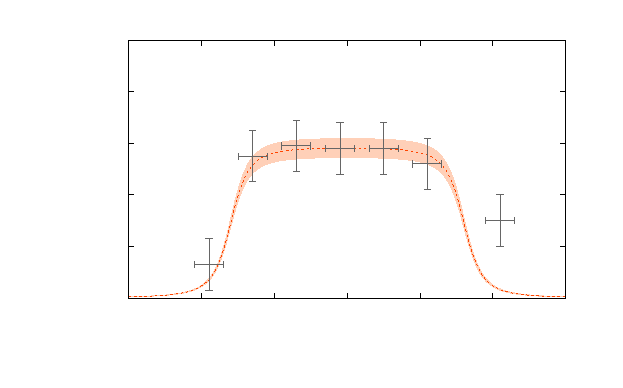
\includegraphics{camp-75-26}}%
    \gplfronttext
  \end{picture}%
\endgroup

	\caption{Camp magnètic al llarg de l'eix d'una bobina de 75 voltes, longitud \SI{16}{cm} i diàmetre \SI{2.6}{cm} per la que hi passa un corrent constant de \SI{1}{A}.}
	\label{fig:camp 75/26}
\end{figure}

\begin{figure}[tp]
	\sffamily \small
	\centering
	% GNUPLOT: LaTeX picture with Postscript
\begingroup
\sffamily \small
  \makeatletter
  \providecommand\color[2][]{%
    \GenericError{(gnuplot) \space\space\space\@spaces}{%
      Package color not loaded in conjunction with
      terminal option `colourtext'%
    }{See the gnuplot documentation for explanation.%
    }{Either use 'blacktext' in gnuplot or load the package
      color.sty in LaTeX.}%
    \renewcommand\color[2][]{}%
  }%
  \providecommand\includegraphics[2][]{%
    \GenericError{(gnuplot) \space\space\space\@spaces}{%
      Package graphicx or graphics not loaded%
    }{See the gnuplot documentation for explanation.%
    }{The gnuplot epslatex terminal needs graphicx.sty or graphics.sty.}%
    \renewcommand\includegraphics[2][]{}%
  }%
  \providecommand\rotatebox[2]{#2}%
  \@ifundefined{ifGPcolor}{%
    \newif\ifGPcolor
    \GPcolortrue
  }{}%
  \@ifundefined{ifGPblacktext}{%
    \newif\ifGPblacktext
    \GPblacktextfalse
  }{}%
  % define a \g@addto@macro without @ in the name:
  \let\gplgaddtomacro\g@addto@macro
  % define empty templates for all commands taking text:
  \gdef\gplbacktext{}%
  \gdef\gplfronttext{}%
  \makeatother
  \ifGPblacktext
    % no textcolor at all
    \def\colorrgb#1{}%
    \def\colorgray#1{}%
  \else
    % gray or color?
    \ifGPcolor
      \def\colorrgb#1{\color[rgb]{#1}}%
      \def\colorgray#1{\color[gray]{#1}}%
      \expandafter\def\csname LTw\endcsname{\color{white}}%
      \expandafter\def\csname LTb\endcsname{\color{black}}%
      \expandafter\def\csname LTa\endcsname{\color{black}}%
      \expandafter\def\csname LT0\endcsname{\color[rgb]{1,0,0}}%
      \expandafter\def\csname LT1\endcsname{\color[rgb]{0,1,0}}%
      \expandafter\def\csname LT2\endcsname{\color[rgb]{0,0,1}}%
      \expandafter\def\csname LT3\endcsname{\color[rgb]{1,0,1}}%
      \expandafter\def\csname LT4\endcsname{\color[rgb]{0,1,1}}%
      \expandafter\def\csname LT5\endcsname{\color[rgb]{1,1,0}}%
      \expandafter\def\csname LT6\endcsname{\color[rgb]{0,0,0}}%
      \expandafter\def\csname LT7\endcsname{\color[rgb]{1,0.3,0}}%
      \expandafter\def\csname LT8\endcsname{\color[rgb]{0.5,0.5,0.5}}%
    \else
      % gray
      \def\colorrgb#1{\color{black}}%
      \def\colorgray#1{\color[gray]{#1}}%
      \expandafter\def\csname LTw\endcsname{\color{white}}%
      \expandafter\def\csname LTb\endcsname{\color{black}}%
      \expandafter\def\csname LTa\endcsname{\color{black}}%
      \expandafter\def\csname LT0\endcsname{\color{black}}%
      \expandafter\def\csname LT1\endcsname{\color{black}}%
      \expandafter\def\csname LT2\endcsname{\color{black}}%
      \expandafter\def\csname LT3\endcsname{\color{black}}%
      \expandafter\def\csname LT4\endcsname{\color{black}}%
      \expandafter\def\csname LT5\endcsname{\color{black}}%
      \expandafter\def\csname LT6\endcsname{\color{black}}%
      \expandafter\def\csname LT7\endcsname{\color{black}}%
      \expandafter\def\csname LT8\endcsname{\color{black}}%
    \fi
  \fi
    \setlength{\unitlength}{0.0500bp}%
    \ifx\gptboxheight\undefined%
      \newlength{\gptboxheight}%
      \newlength{\gptboxwidth}%
      \newsavebox{\gptboxtext}%
    \fi%
    \setlength{\fboxrule}{0.5pt}%
    \setlength{\fboxsep}{1pt}%
\begin{picture}(5668.00,3400.00)%
    \gplgaddtomacro\gplbacktext{%
      \csname LTb\endcsname%%
      \put(946,704){\makebox(0,0)[r]{\strut{}\num{0}}}%
      \put(946,1323){\makebox(0,0)[r]{\strut{}\num{0.5}}}%
      \put(946,1942){\makebox(0,0)[r]{\strut{}\num{1}}}%
      \put(946,2560){\makebox(0,0)[r]{\strut{}\num{1.5}}}%
      \put(946,3179){\makebox(0,0)[r]{\strut{}\num{2}}}%
      \put(1078,484){\makebox(0,0){\strut{}\num{-15}}}%
      \put(1777,484){\makebox(0,0){\strut{}\num{-10}}}%
      \put(2476,484){\makebox(0,0){\strut{}\num{-5}}}%
      \put(3175,484){\makebox(0,0){\strut{}\num{0}}}%
      \put(3873,484){\makebox(0,0){\strut{}\num{5}}}%
      \put(4572,484){\makebox(0,0){\strut{}\num{10}}}%
      \put(5271,484){\makebox(0,0){\strut{}\num{15}}}%
    }%
    \gplgaddtomacro\gplfronttext{%
      \csname LTb\endcsname%%
      \put(198,1941){\rotatebox{-270}{\makebox(0,0){\strut{}$\mathsf{B \ (\si{mT})}$}}}%
      \put(3174,154){\makebox(0,0){\strut{}$\mathsf{z \ (\si{cm})}$}}%
    }%
    \gplbacktext
    \put(0,0){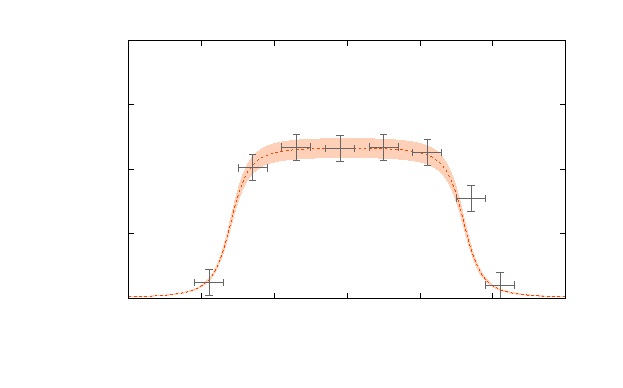
\includegraphics{camp-150-26}}%
    \gplfronttext
  \end{picture}%
\endgroup

	\caption{Camp magnètic al llarg de l'eix d'una bobina de 150 voltes, longitud \SI{16}{cm} i diàmetre \SI{2.6}{cm} per la que hi passa un corrent constant de \SI{1}{A}.}
	\label{fig:camp 150/26}
\end{figure}

\begin{figure}[tp]
	\sffamily \small
	\centering
	% GNUPLOT: LaTeX picture with Postscript
\begingroup
\sffamily \small
  \makeatletter
  \providecommand\color[2][]{%
    \GenericError{(gnuplot) \space\space\space\@spaces}{%
      Package color not loaded in conjunction with
      terminal option `colourtext'%
    }{See the gnuplot documentation for explanation.%
    }{Either use 'blacktext' in gnuplot or load the package
      color.sty in LaTeX.}%
    \renewcommand\color[2][]{}%
  }%
  \providecommand\includegraphics[2][]{%
    \GenericError{(gnuplot) \space\space\space\@spaces}{%
      Package graphicx or graphics not loaded%
    }{See the gnuplot documentation for explanation.%
    }{The gnuplot epslatex terminal needs graphicx.sty or graphics.sty.}%
    \renewcommand\includegraphics[2][]{}%
  }%
  \providecommand\rotatebox[2]{#2}%
  \@ifundefined{ifGPcolor}{%
    \newif\ifGPcolor
    \GPcolortrue
  }{}%
  \@ifundefined{ifGPblacktext}{%
    \newif\ifGPblacktext
    \GPblacktextfalse
  }{}%
  % define a \g@addto@macro without @ in the name:
  \let\gplgaddtomacro\g@addto@macro
  % define empty templates for all commands taking text:
  \gdef\gplbacktext{}%
  \gdef\gplfronttext{}%
  \makeatother
  \ifGPblacktext
    % no textcolor at all
    \def\colorrgb#1{}%
    \def\colorgray#1{}%
  \else
    % gray or color?
    \ifGPcolor
      \def\colorrgb#1{\color[rgb]{#1}}%
      \def\colorgray#1{\color[gray]{#1}}%
      \expandafter\def\csname LTw\endcsname{\color{white}}%
      \expandafter\def\csname LTb\endcsname{\color{black}}%
      \expandafter\def\csname LTa\endcsname{\color{black}}%
      \expandafter\def\csname LT0\endcsname{\color[rgb]{1,0,0}}%
      \expandafter\def\csname LT1\endcsname{\color[rgb]{0,1,0}}%
      \expandafter\def\csname LT2\endcsname{\color[rgb]{0,0,1}}%
      \expandafter\def\csname LT3\endcsname{\color[rgb]{1,0,1}}%
      \expandafter\def\csname LT4\endcsname{\color[rgb]{0,1,1}}%
      \expandafter\def\csname LT5\endcsname{\color[rgb]{1,1,0}}%
      \expandafter\def\csname LT6\endcsname{\color[rgb]{0,0,0}}%
      \expandafter\def\csname LT7\endcsname{\color[rgb]{1,0.3,0}}%
      \expandafter\def\csname LT8\endcsname{\color[rgb]{0.5,0.5,0.5}}%
    \else
      % gray
      \def\colorrgb#1{\color{black}}%
      \def\colorgray#1{\color[gray]{#1}}%
      \expandafter\def\csname LTw\endcsname{\color{white}}%
      \expandafter\def\csname LTb\endcsname{\color{black}}%
      \expandafter\def\csname LTa\endcsname{\color{black}}%
      \expandafter\def\csname LT0\endcsname{\color{black}}%
      \expandafter\def\csname LT1\endcsname{\color{black}}%
      \expandafter\def\csname LT2\endcsname{\color{black}}%
      \expandafter\def\csname LT3\endcsname{\color{black}}%
      \expandafter\def\csname LT4\endcsname{\color{black}}%
      \expandafter\def\csname LT5\endcsname{\color{black}}%
      \expandafter\def\csname LT6\endcsname{\color{black}}%
      \expandafter\def\csname LT7\endcsname{\color{black}}%
      \expandafter\def\csname LT8\endcsname{\color{black}}%
    \fi
  \fi
    \setlength{\unitlength}{0.0500bp}%
    \ifx\gptboxheight\undefined%
      \newlength{\gptboxheight}%
      \newlength{\gptboxwidth}%
      \newsavebox{\gptboxtext}%
    \fi%
    \setlength{\fboxrule}{0.5pt}%
    \setlength{\fboxsep}{1pt}%
\begin{picture}(5668.00,3400.00)%
    \gplgaddtomacro\gplbacktext{%
      \csname LTb\endcsname%%
      \put(946,704){\makebox(0,0)[r]{\strut{}\num{0}}}%
      \put(946,1013){\makebox(0,0)[r]{\strut{}\num{0.5}}}%
      \put(946,1323){\makebox(0,0)[r]{\strut{}\num{1}}}%
      \put(946,1632){\makebox(0,0)[r]{\strut{}\num{1.5}}}%
      \put(946,1942){\makebox(0,0)[r]{\strut{}\num{2}}}%
      \put(946,2251){\makebox(0,0)[r]{\strut{}\num{2.5}}}%
      \put(946,2560){\makebox(0,0)[r]{\strut{}\num{3}}}%
      \put(946,2870){\makebox(0,0)[r]{\strut{}\num{3.5}}}%
      \put(946,3179){\makebox(0,0)[r]{\strut{}\num{4}}}%
      \put(1078,484){\makebox(0,0){\strut{}\num{-15}}}%
      \put(1777,484){\makebox(0,0){\strut{}\num{-10}}}%
      \put(2476,484){\makebox(0,0){\strut{}\num{-5}}}%
      \put(3175,484){\makebox(0,0){\strut{}\num{0}}}%
      \put(3873,484){\makebox(0,0){\strut{}\num{5}}}%
      \put(4572,484){\makebox(0,0){\strut{}\num{10}}}%
      \put(5271,484){\makebox(0,0){\strut{}\num{15}}}%
    }%
    \gplgaddtomacro\gplfronttext{%
      \csname LTb\endcsname%%
      \put(198,1941){\rotatebox{-270}{\makebox(0,0){\strut{}$\mathsf{B \ (\si{mT})}$}}}%
      \put(3174,154){\makebox(0,0){\strut{}$\mathsf{z \ (\si{cm})}$}}%
    }%
    \gplbacktext
    \put(0,0){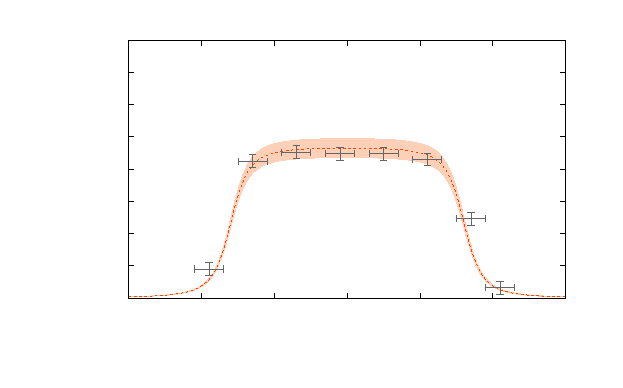
\includegraphics{camp-300-26}}%
    \gplfronttext
  \end{picture}%
\endgroup

	\caption{Camp magnètic al llarg de l'eix d'una bobina de 300 voltes, longitud \SI{16}{cm} i diàmetre \SI{2.6}{cm} per la que hi passa un corrent constant de \SI{1}{A}.}
	\label{fig:camp 300/26}
\end{figure}

A les \cref{fig:camp 300/33,fig:camp 75/26,fig:camp 150/26,fig:camp 300/26} hi ha representat el mòdul del camp magnètic al llarg de l'eix de les bobines mesurades durant l'experiment---calculat a partir de l'\cref{eq:camp bobina} i amb el corresponent marge d'incertesa--- aixì com els punts corresponents a les mesures realitzades

Tal i com es pot apreciar, al llarg de l'eix les mesures obtingudes s'ajusten molt bé a la prediccío teòrica. Això és d'esperar ja que a l'interior d'una bobina el camp és pràcticament constant. Als extrems, però, les dades experimentals no s'hi ajusten tant. Una explicació és que en  

\section{Conclusions}
En general els resultats obtinguts han estat satisfactoris. S'ha observat empíricament al llarg de tota la pràctica els fets que s'havien demostrat de manera teòrica. El camp magnètic al centre d'una espira disminueix a mesura que augmenta el radi d'aquesta i ho fa com $\frac{1}{R}$ amb $R$ el radi de l'espira. S'ha comprovat també empíricament l'augment lineal del camp al centre d'un conjunt d'espires amb la quantitat d'espires. Aquest últim fet ha estat provat per conjunts de $1$, $2$ i $3$ espires. Les observacions han portat també a concloure que el camp magnètic al centre d'una bobina augmenta en apropar-se al centre i és màxim en aquest. El fet que el camp magnètic creat per una bobina on hi circula una certa intensitat augmenta amb el nombre de voltes, ha estat provat també de manera satisfactòria. Finalment s'ha calculat empíricament la permeabilitat magnètica $\mu_{0}$ i s'ha obtingut una bona aproximació d'aquesta.






% Annexos
\addcontentsline{toc}{part}{Annexos}
\appendix
\titleformat{\chapter}[display]{\centering \bfseries \sffamily \LARGE}{\large \sf Annex \thechapter}{4pt}{}{}
\titlespacing{\chapter}{0pt}{*2}{*4}

\chapter{Annexos}
\section{Annex}
\todo{S'ha de decidir l'estructura dels annexos}
\begin{table}
	\centering
	\sffamily \small
	\caption{Mesures de la intensitat necessària per contrarrestar la força gravitatòria de cada massa}
	\label{tab:forca v intensitat (detall)}

	\todo[inline]{No sé com fer aquesta taula}

	\begin{tabular}{SSSSS}
		\toprule	
		\multicolumn{5}{c}{Massa (\si{mg})} \\
		{5} & {10} & {15} & {20} & {25} \\
		\midrule 
		2.62 & 3.70 & 4.47 & 5.10 & 6.05 \\
		2.55 & 3.40 & 4.46 & 5.29 & 5.99 \\
		2.65 & 3.58 & 4.63 & 5.33 & 5.94 \\
		2.62 & 3.64 & 4.42 & 5.07 & 5.40 \\
		2.60 & 3.71 & 4.50 & 5.10 & 5.21 \\
		2.57 & 3.68 & 4.48 & 5.11 & 5.63 \\
		\bottomrule
	\end{tabular}
\end{table}


\begin{table}
	\centering
	\sffamily
	\small
	\caption{Dades de la regressió lineal entre la força del fil de torsió i la rotació del dial}
	\label{tab:regressio forca-angle}

	\begin{tabular}{SS}
		\toprule
		{Mass (\si{mg})} & {Rotació (\si{\degree}) (\( {} \pm \SI{1}{\degree} \))} \\
		\midrule
		5 & 13 \\
		10 & 27 \\
		15 & 44 \\
		20 & 63 \\
		25 & 70 \\
		\bottomrule
	\end{tabular}
\end{table}

\begin{figure}
	\centering
	% GNUPLOT: LaTeX picture with Postscript
\begingroup
\sffamily \small
  \makeatletter
  \providecommand\color[2][]{%
    \GenericError{(gnuplot) \space\space\space\@spaces}{%
      Package color not loaded in conjunction with
      terminal option `colourtext'%
    }{See the gnuplot documentation for explanation.%
    }{Either use 'blacktext' in gnuplot or load the package
      color.sty in LaTeX.}%
    \renewcommand\color[2][]{}%
  }%
  \providecommand\includegraphics[2][]{%
    \GenericError{(gnuplot) \space\space\space\@spaces}{%
      Package graphicx or graphics not loaded%
    }{See the gnuplot documentation for explanation.%
    }{The gnuplot epslatex terminal needs graphicx.sty or graphics.sty.}%
    \renewcommand\includegraphics[2][]{}%
  }%
  \providecommand\rotatebox[2]{#2}%
  \@ifundefined{ifGPcolor}{%
    \newif\ifGPcolor
    \GPcolortrue
  }{}%
  \@ifundefined{ifGPblacktext}{%
    \newif\ifGPblacktext
    \GPblacktextfalse
  }{}%
  % define a \g@addto@macro without @ in the name:
  \let\gplgaddtomacro\g@addto@macro
  % define empty templates for all commands taking text:
  \gdef\gplbacktext{}%
  \gdef\gplfronttext{}%
  \makeatother
  \ifGPblacktext
    % no textcolor at all
    \def\colorrgb#1{}%
    \def\colorgray#1{}%
  \else
    % gray or color?
    \ifGPcolor
      \def\colorrgb#1{\color[rgb]{#1}}%
      \def\colorgray#1{\color[gray]{#1}}%
      \expandafter\def\csname LTw\endcsname{\color{white}}%
      \expandafter\def\csname LTb\endcsname{\color{black}}%
      \expandafter\def\csname LTa\endcsname{\color{black}}%
      \expandafter\def\csname LT0\endcsname{\color[rgb]{1,0,0}}%
      \expandafter\def\csname LT1\endcsname{\color[rgb]{0,1,0}}%
      \expandafter\def\csname LT2\endcsname{\color[rgb]{0,0,1}}%
      \expandafter\def\csname LT3\endcsname{\color[rgb]{1,0,1}}%
      \expandafter\def\csname LT4\endcsname{\color[rgb]{0,1,1}}%
      \expandafter\def\csname LT5\endcsname{\color[rgb]{1,1,0}}%
      \expandafter\def\csname LT6\endcsname{\color[rgb]{0,0,0}}%
      \expandafter\def\csname LT7\endcsname{\color[rgb]{1,0.3,0}}%
      \expandafter\def\csname LT8\endcsname{\color[rgb]{0.5,0.5,0.5}}%
    \else
      % gray
      \def\colorrgb#1{\color{black}}%
      \def\colorgray#1{\color[gray]{#1}}%
      \expandafter\def\csname LTw\endcsname{\color{white}}%
      \expandafter\def\csname LTb\endcsname{\color{black}}%
      \expandafter\def\csname LTa\endcsname{\color{black}}%
      \expandafter\def\csname LT0\endcsname{\color{black}}%
      \expandafter\def\csname LT1\endcsname{\color{black}}%
      \expandafter\def\csname LT2\endcsname{\color{black}}%
      \expandafter\def\csname LT3\endcsname{\color{black}}%
      \expandafter\def\csname LT4\endcsname{\color{black}}%
      \expandafter\def\csname LT5\endcsname{\color{black}}%
      \expandafter\def\csname LT6\endcsname{\color{black}}%
      \expandafter\def\csname LT7\endcsname{\color{black}}%
      \expandafter\def\csname LT8\endcsname{\color{black}}%
    \fi
  \fi
    \setlength{\unitlength}{0.0500bp}%
    \ifx\gptboxheight\undefined%
      \newlength{\gptboxheight}%
      \newlength{\gptboxwidth}%
      \newsavebox{\gptboxtext}%
    \fi%
    \setlength{\fboxrule}{0.5pt}%
    \setlength{\fboxsep}{1pt}%
\begin{picture}(5668.00,3400.00)%
    \gplgaddtomacro\gplbacktext{%
      \csname LTb\endcsname%%
      \put(1078,704){\makebox(0,0)[r]{\strut{}\num{0}}}%
      \put(1078,1117){\makebox(0,0)[r]{\strut{}\num{0.05}}}%
      \put(1078,1529){\makebox(0,0)[r]{\strut{}\num{0.1}}}%
      \put(1078,1942){\makebox(0,0)[r]{\strut{}\num{0.15}}}%
      \put(1078,2354){\makebox(0,0)[r]{\strut{}\num{0.2}}}%
      \put(1078,2767){\makebox(0,0)[r]{\strut{}\num{0.25}}}%
      \put(1078,3179){\makebox(0,0)[r]{\strut{}\num{0.3}}}%
      \put(1210,484){\makebox(0,0){\strut{}\num{10}}}%
      \put(1790,484){\makebox(0,0){\strut{}\num{20}}}%
      \put(2370,484){\makebox(0,0){\strut{}\num{30}}}%
      \put(2950,484){\makebox(0,0){\strut{}\num{40}}}%
      \put(3531,484){\makebox(0,0){\strut{}\num{50}}}%
      \put(4111,484){\makebox(0,0){\strut{}\num{60}}}%
      \put(4691,484){\makebox(0,0){\strut{}\num{70}}}%
      \put(5271,484){\makebox(0,0){\strut{}\num{80}}}%
    }%
    \gplgaddtomacro\gplfronttext{%
      \csname LTb\endcsname%%
      \put(198,1941){\rotatebox{-270}{\makebox(0,0){\strut{}$\mathsf{F \ (\si{mN})}$}}}%
      \put(3240,154){\makebox(0,0){\strut{}$\mathsf{\theta \ (\si{\degree})}$}}%
    }%
    \gplbacktext
    \put(0,0){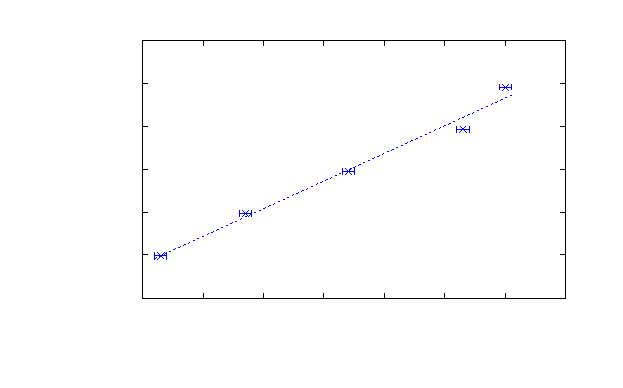
\includegraphics{forca-rotacio}}%
    \gplfronttext
  \end{picture}%
\endgroup

	\caption{Força en funció de la rotació del dial}
	\label{fig:força v rotacio}
\end{figure}



\end{document}

